
\chapter{Data and Data Pre-Processing}
\section{About Dataset}
\subsection{Content}
In this Dataset, we have information about economic data of UK from 1960 to 2021. \\

\textbf{GDP per capita (current US\$)} \\
Gross domestic product divided by midyear population equals GDP per capita. GDP is calculated as the total gross value added by all producers who are residents of the economy, plus any applicable product taxes, less any subsidies that are not reflected in the prices of the goods. It is estimated without taking into account natural resource deterioration or the depreciation of manufactured assets. The currency used for the data is the current dollar. \\


\textbf{GDP growth (annual \%)}\\
GDP annual percentage growth rate based on constant local currency pricing. The aggregates are based on 2015 prices that are constant and expressed in US dollars. GDP is calculated as the total gross value added by all producers who are residents of the economy, plus any applicable product taxes, minus any unaccounted-for subsidies. It is estimated without taking into account the deterioration and depletion of natural resources or the depreciation of manufactured assets.\\

\textbf{Unemployment, total (\% of total labor force) (modeled ILO estimate)}\\
The percentage of the labour force that is unemployed yet looking for work is referred to as unemployment.\\

\textbf{Inflation, consumer prices (annual \%)}\\
The cost of procuring a basket of goods and services for the average consumer may be fixed or altered at predetermined periods, such as annually, and is reflected in inflation as measured by the consumer price index. Typically, the Laspeyres formula is applied.\\

\textbf{Personal remittances, received (\% of GDP)}\\
Personal transfers and employee remuneration are included in personal remittances. All recent financial or in-kind transfers made or received by resident households to or from nonresident households are referred to as personal transfers. Thus, any recent transactions between residents and non-residents are considered personal transfers. The income of border, seasonal, and other short-term workers who labour in an economy where they are not residents, as well as of residents employed by nonresident businesses, is referred to as compensation of employees. Data are the sum of two components, personal transfers and employee compensation, as defined in the sixth edition of the IMF's Balance of Payments Manual.\\

\subsection{Dataset Glossary}
\begin{table}[ht]
\centering
\caption{Dataset Information}
\label{tab2}
\begin{tabular}{llllllll}
 \hline
Column Name & Description & wbdata search indicator\\
\hline
 gdp-p-capita & info & NY.GDP.PCAP.PP.CD \\
 inflation-cpi & info & FP.CPI.TOTL.ZG \\
 gdp-growth & GDP growth percentage of each year & NY.GDP.MKTP.KD.ZG \\
 unemp-total & info & SL.UEM.TOTL.ZS \\
 p-remittances & info & BX.TRF.PWKR.DT.GD.ZS \\
\hline
\end{tabular}
\end{table}

\subsection{Structure of the Dataset}
\begin{tabular}{rrrrr}
\toprule
 gdp-p-capita &  inflation-cpi &  gdp-growth &  unemp-total &  p-remittances \\
 \midrule
 49675.304674 &       2.518371 &    7.441273 &                4.526 &                   NaN \\
 46526.911865 &       0.989487 &   -9.270411 &                4.472 &              0.117817 \\
 49041.463548 &       1.738105 &    1.671944 &                3.740 &              0.146415 \\
 47573.488016 &       2.292840 &    1.650925 &                4.000 &              0.151328 \\
 46372.386604 &       2.557756 &    2.134453 &                4.330 &              0.159551 \\
\bottomrule
\end{tabular}

\subsection{Python Script to fetch Dataset}
\begin{lstlisting}[language=Python]
# python script to fetch data from world bank data
# wbdata library to fetch data from world bank data before running you need to install in wbdata, pandas,numpy 


import wbdata
import pandas as pd, numpy as np
import os

#create a Python list of the countries for which you would like to download data.
## use the wbdata.get_country() command to see a list of country abbreviations for the wbdata dataset

selcountries=['GBR']


#wbdata.search_indicators("GDP per capita") to get indicator for fetching data from worldbank data
#create a Python dictionary with the identifiers of the wbdata variables you would like to use, assigning to each a more common-sense name for each variable
economic_data={
            "NY.GDP.PCAP.PP.CD":"gdp-p-capita", 
            "FP.CPI.TOTL.ZG":"inflation-cpi",
            "NY.GDP.MKTP.KD.ZG":"gdp-growth",
            "SL.UEM.TOTL.ZS":"unemp-total",
            "BX.TRF.PWKR.DT.GD.ZS":"p-remittances"
        }


#assign the above dictionary of variables to a new name
indicators = economic_data

#download data from wbdata given the countries and variables listed above
df=wbdata.get_dataframe(indicators,country=selcountries)

# saving the dataframe
df.to_csv('data.csv')

df.head()

\end{lstlisting}


\section{Cleaning and Understanding Time Series Data}

\subsection{Context}

\hspace{10mm}Making meaning of the dataset and cleaning it are always essential for success, regardless of the type of data science project to which one is assigned. Exploratory data analysis (EDA) is the initial stage in understanding the data since it enables us to develop a logical strategy for resolving the business issue. It also enables us to spot problems like outliers that are present in our dataset.

Before conducting any analysis, these problems must be resolved because if our data is inaccurate, so will the analysis. Additionally, because the conclusions of such a study won't align with our clients' theoretical or professional expertise, they can lose faith in our work. Even if the clients choose to act as a result of such analysis, the outcome will be incorrect, and we will be in big trouble! Therefore, the quality of the outcomes is greatly influenced by how effectively we clean and comprehend the data.

When working with datasets that have hidden qualities, such as time series datasets, things become a little bit more difficult. Time series datasets are a unique kind of data that are arranged chronologically and require particular care when handling their inherent components, such as trend and seasonality.

\subsection{Theory: About Time Series Data}

\hspace{10mm}A set of numbers and information about the dates on which those numbers were recorded make up a time-series data. A time series is most frequently a sequence captured at a series of equally spaced moments in time. The four components of time series data are as follows:

\textbf{Trend:} The trend in a time series is the long-term pattern. Depending on whether the time series exhibits a rising long-term pattern or a declining long-term pattern, a trend may be positive or negative.

\textbf{Seasonal:} Represents changes that occur at predictable, defined intervals (i.e. factors like time of the year). The rise in retail sales over the Christmas season and the subsequent drop can serve as an illustration.


\textbf{Cyclical:}A cyclical pattern is any pattern that exhibits an upward and downward movement around a specific trend. The sort of business or industry being studied determines the cycle's length.


\textbf{Irregular:}The variation in the variable under study is caused by another factor. They are merely random or irregular variations, not regular variations. These variations are chaotic, unanticipated, unmanageable, and unforeseeable. Earthquakes, wars, floods, famines, and other natural disasters are examples of these forces.


\vspace{10mm}

We can extract the trend, seasonality, and error/irregularity components of a time series dataset using decomposition techniques. There are other decomposition approaches, but in this project's EDA section, we'll concentrate on the additive approach. \\

\vspace{5mm}
\textbf{Stationary} \\
A stationary time series is one whose characteristics do not change depending on the time at which the series is seen. As a result, time series containing trends or seasonality are not stationary since the trend and seasonality will change the time series' value over time.

\begin{figure}[H]
    \centering
    
\includegraphics[width=0.7\textwidth]{Images/stati.png}
    \caption{}
    \label{fig1}
\end{figure}

What is this property so crucial? Since the way stationary processes change is predictable and steady, modelling stationary processes is simpler. Most time series models need us to check whether the data was produced by a stationary process; if not, we may need to change it to give it the characteristics of a stationary process.



\vspace{5mm}
\textbf{ACF and PACF} \\
To determine stationarity and time series model parameters, autocorrelation (ACF) and partial autocorrelation (PACF) plots are frequently utilised. These graphs illustrate the consistency of a link between an observation and an observation in a time series with observations at earlier time steps.

We determine the connection between time-series observations and earlier time steps, referred to as lags, for ACF plots. The relationship between an observation in a time series and observations at earlier time steps, without the relationships of intervening observations, is summarised by the PACF plot. Within the first few lags, such time graphs for a stationary process start to show statistically insignificant values.

\subsection{Data Cleaning: Handling missing value and outliers}


\begin{lstlisting}[language=Python]
# python script for Data Cleaning Section
# importing required libraries
import numpy as np
import seaborn as sns
from matplotlib import pyplot as plt
from statsmodels.tsa.stattools import adfuller
from statsmodels.graphics.tsaplots import plot_acf
from statsmodels.graphics.tsaplots import plot_pacf
from pandas import datetime
from statsmodels.tsa.arima_model import ARIMA
from statsmodels.tsa.arima_model import ARMA
from sklearn.metrics import mean_squared_error
from statsmodels.tsa.seasonal import seasonal_decompose
plt.rcParams["figure.figsize"] = (30,5)

# function to display shape, data type, data near head and tail of given data fram.
# Input Arguments df: dataframe, n: No f data points to display
def df_details(d_f,n):
    print('Data Types of Column: \n',d_f.dtypes)
    print('\n Size of Datarame: ',d_f.shape)
    print('\n Top and bottom ',n,' rows: \n')
    display(d_f.head(n).append(d_f.tail(n)))

df_details(df,5) 


# Understanding the numeric fields
df.describe()


# Histogram of all numeric fields
df_hist = df
df_hist.hist(figsize=(15,15));

df2 = df
df2['tmp'] = df.index
df2.info()

# function to plot graph Year v/s differen column
df2 = df
df2['tmp'] = df.index

def plot_graph(df):
  plt.rcParams["figure.figsize"] = (30,5)
  col = list(df.columns)
  for columnName in col:
    if columnName != 'tmp':
      plt.plot(df['tmp'],df[columnName])
      plt.xlabel("Year")
      plt.ylabel(columnName)
      plt.show()



plot_graph(df2)

#check missing value in data 
def missing_value(d_f):
    print('Available data with no nulls: ', d_f.dropna().shape[0])
    display('Deatils of Null values column wise',d_f.isnull().sum())


missing_value(df2)

# This function fill missing values
def fill_miss(d_f,metd = None):
    col_name = d_f.columns
    av_method = ['bfill', 'pad', 'ffill', 'linear','mean']

    if metd == None:
        return d_f
    for col in col_name:    
      if (metd == 'mean'):
          d_f[col] = d_f[col].fillna(value=d_f[col].mean()) 
      elif metd == 'linear':
          d_f[col] = d_f[col].interpolate(method = 'linear') 
      elif  metd in av_method:
          d_f[col] = d_f[col].fillna(method = metd)
      else:
          print("Invalid fill type")
          return d_f

fill_miss(df2, 'ffill')
fill_miss(df2, 'bfill')
missing_value(df2)          

# Outlier Detection using Inter Quartile Range
def out_iqr(s, k=1.5, return_thresholds=False):
    """
    Return a boolean mask of outliers for a series
    using interquartile range, works column-wise.
    param k:
        some cutoff to multiply by the iqr
    :type k: ``float``
    param return_thresholds:
        True returns the lower and upper bounds, good for plotting.
        False returns the masked array 
    :type return_thresholds: ``bool``
    """
    # calculate interquartile range
    q25, q75 = np.percentile(s, 25), np.percentile(s, 75)
    iqr = q75 - q25
    # calculate the outlier cutoff
    cut_off = iqr * k
    lower, upper = q25 - cut_off, q75 + cut_off
    if return_thresholds:
        return lower, upper
    else: # identify outliers
        return [True if x < lower or x > upper else False for x in s]
    
    
# For comparison, make one array each at varying values of k.
df3 = df2.drop(columns=['tmp'],axis=1)
iqr1 = df3.apply(out_iqr, k=1.5)
iqr1.head(10)

for column in df3:
    df3[column] = np.where(iqr1[column] == True,'NaN',df3[column])
cols = df3.columns
df3[cols] = df3[cols].apply(pd.to_numeric, errors='coerce')
df3.head(10)

#Use linear interpolation to fill up nulls
df3 = df3.interpolate(method='linear', axis=0).bfill().ffill()
df3.head()

#checking for missing value after outlier correction
df4 = df3
df4['tmp'] = df3.index
missing_value(df4)

\end{lstlisting}

\textbf{Plot: Target Variable vs Year}\\

\begin{figure}[H]
    \centering
    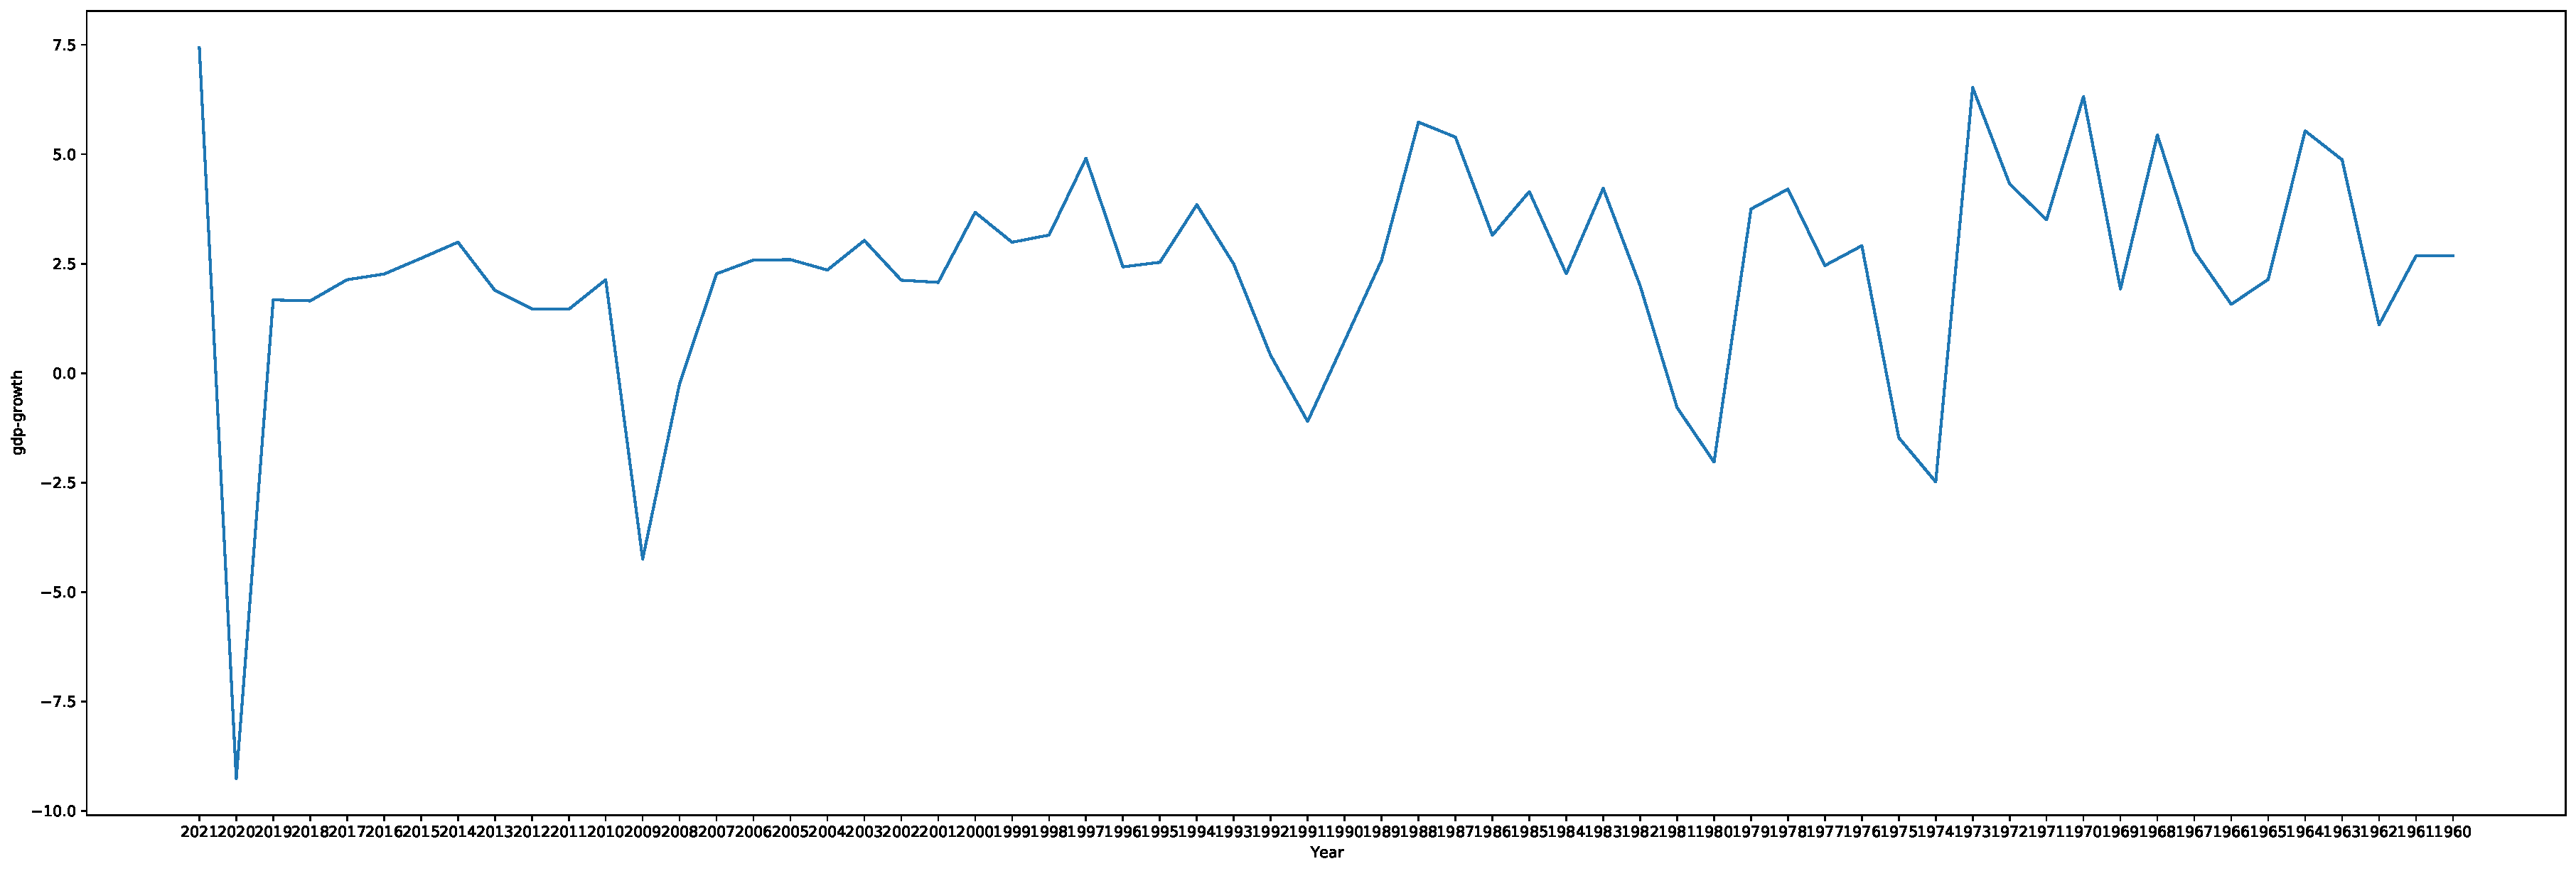
\includegraphics[width=0.7\textwidth]{Images/gdp-growth vs year (1).pdf}
    \caption{GDP Growth}
    \label{fig1}
\end{figure}


\begin{figure}[H]
    \centering
    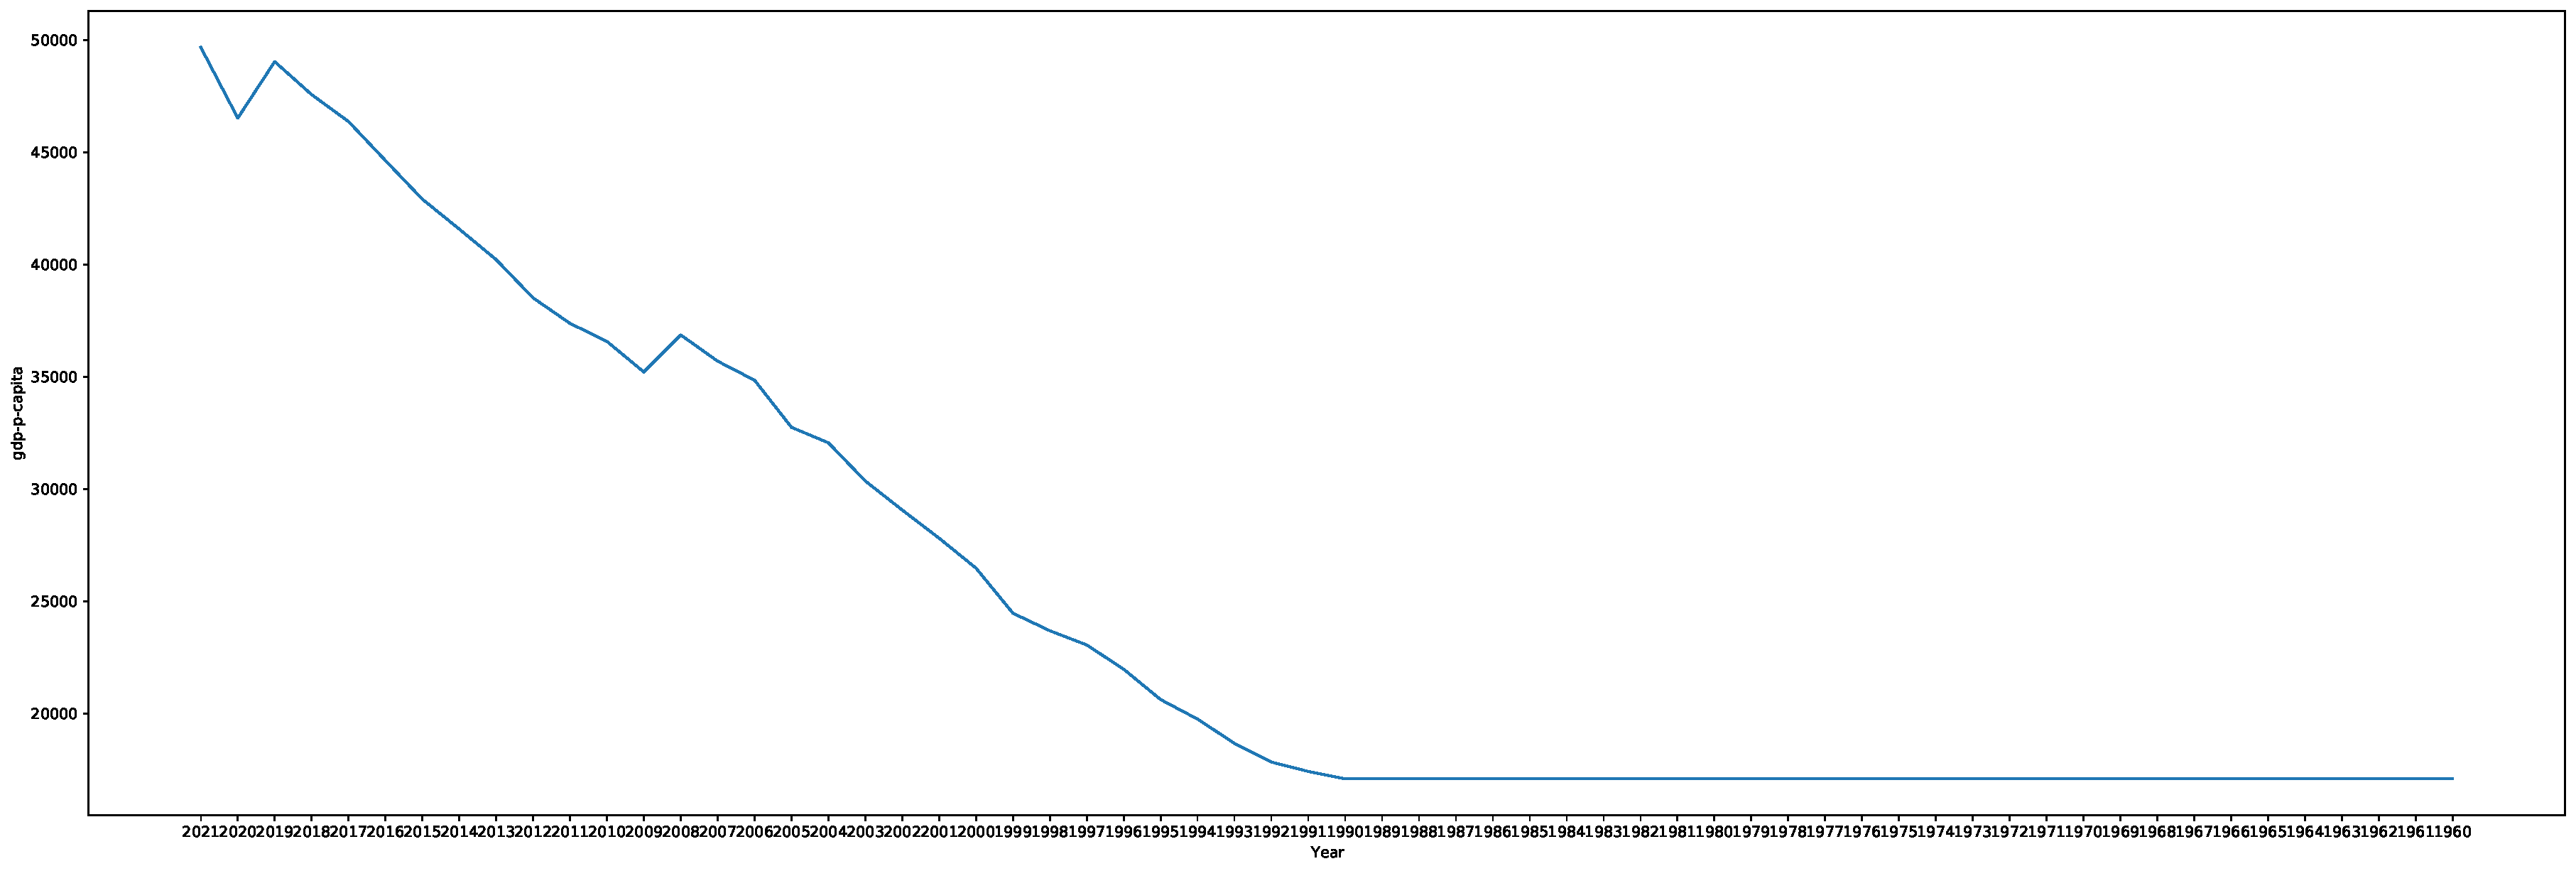
\includegraphics[width=0.7\textwidth]{Images/gdp-p-capita vs year (1).pdf}
    \caption{GDP Person Capita}
    \label{fig1}
\end{figure}

\begin{figure}[H]
    \centering
    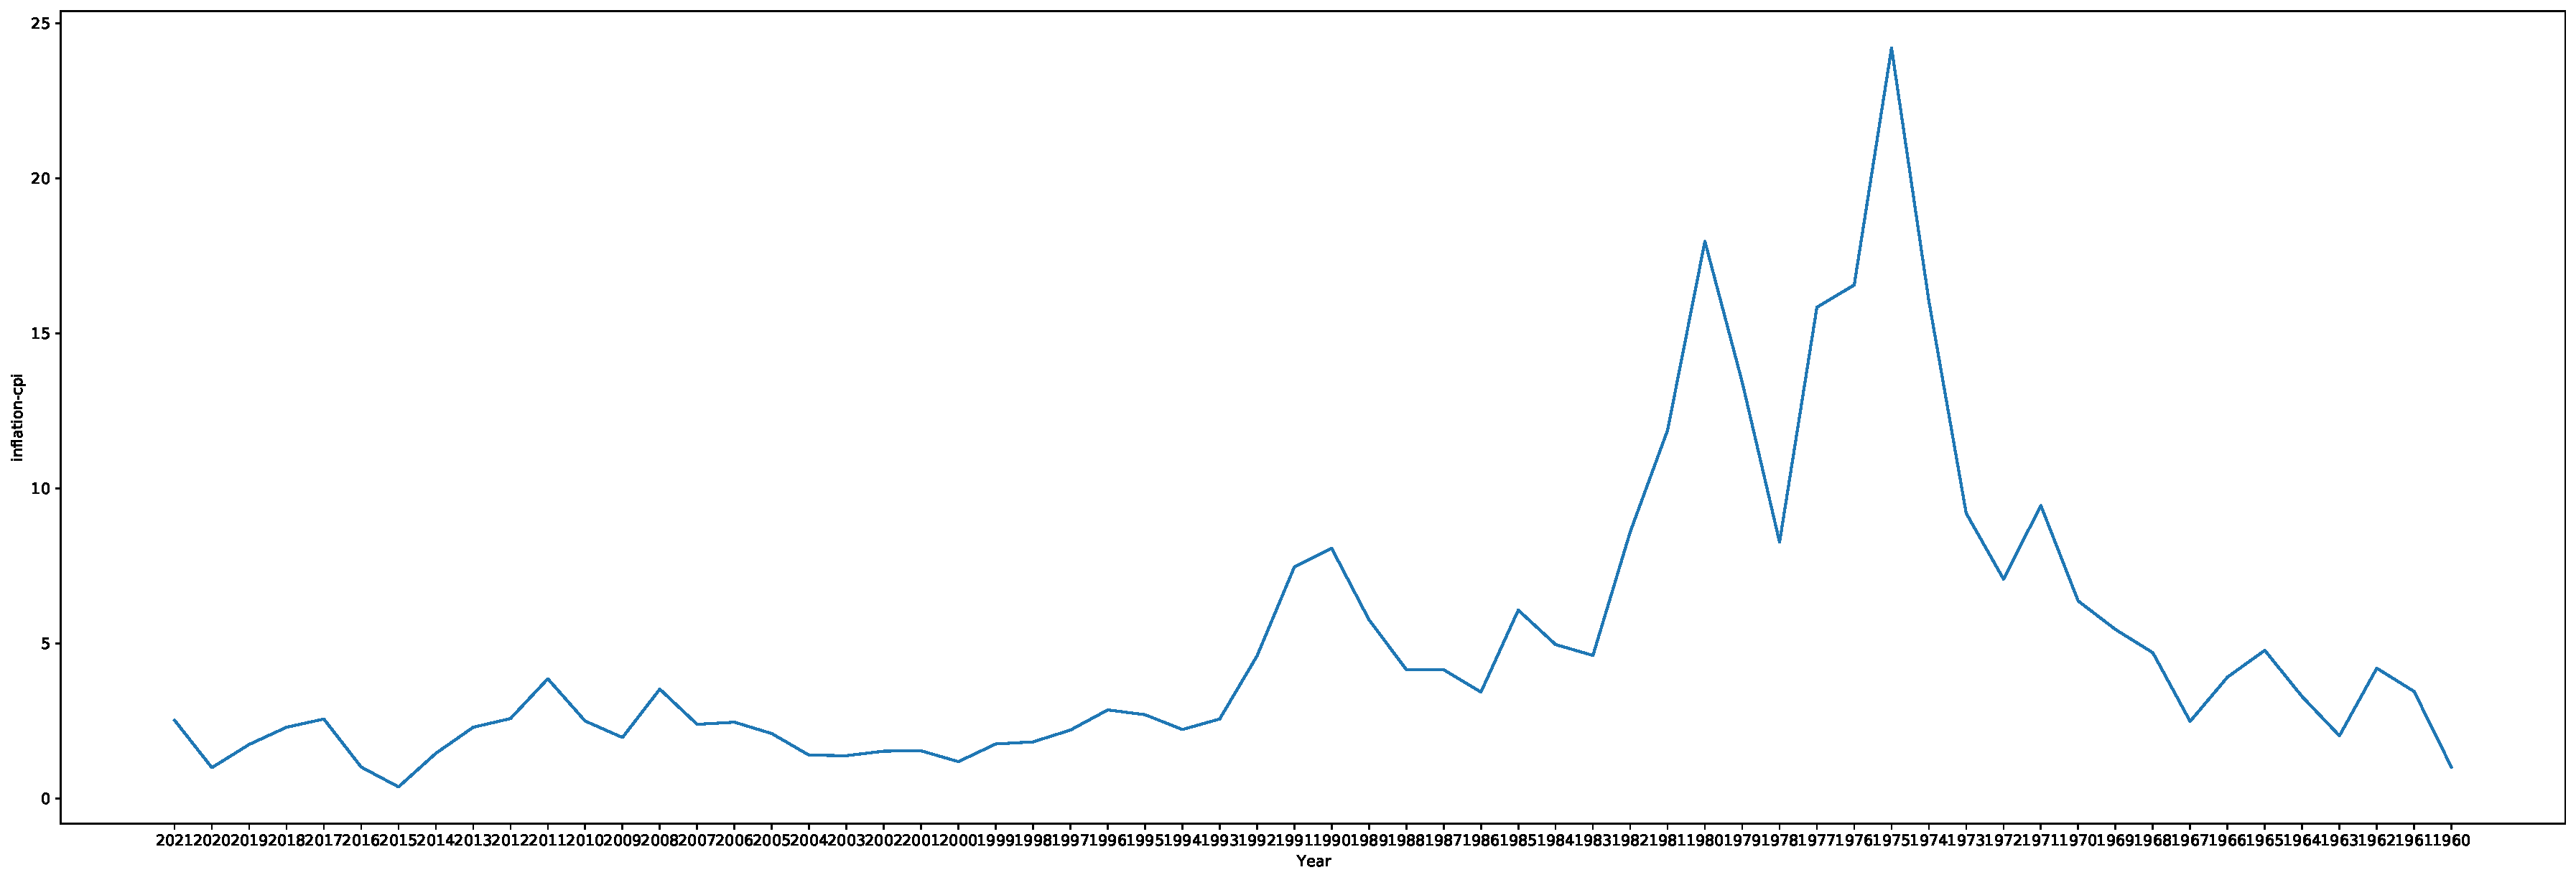
\includegraphics[width=0.7\textwidth]{Images/inflation-cpi vs year (1).pdf}
    \caption{Inflation}
    \label{fig1}
\end{figure}

\begin{figure}[H]
    \centering
    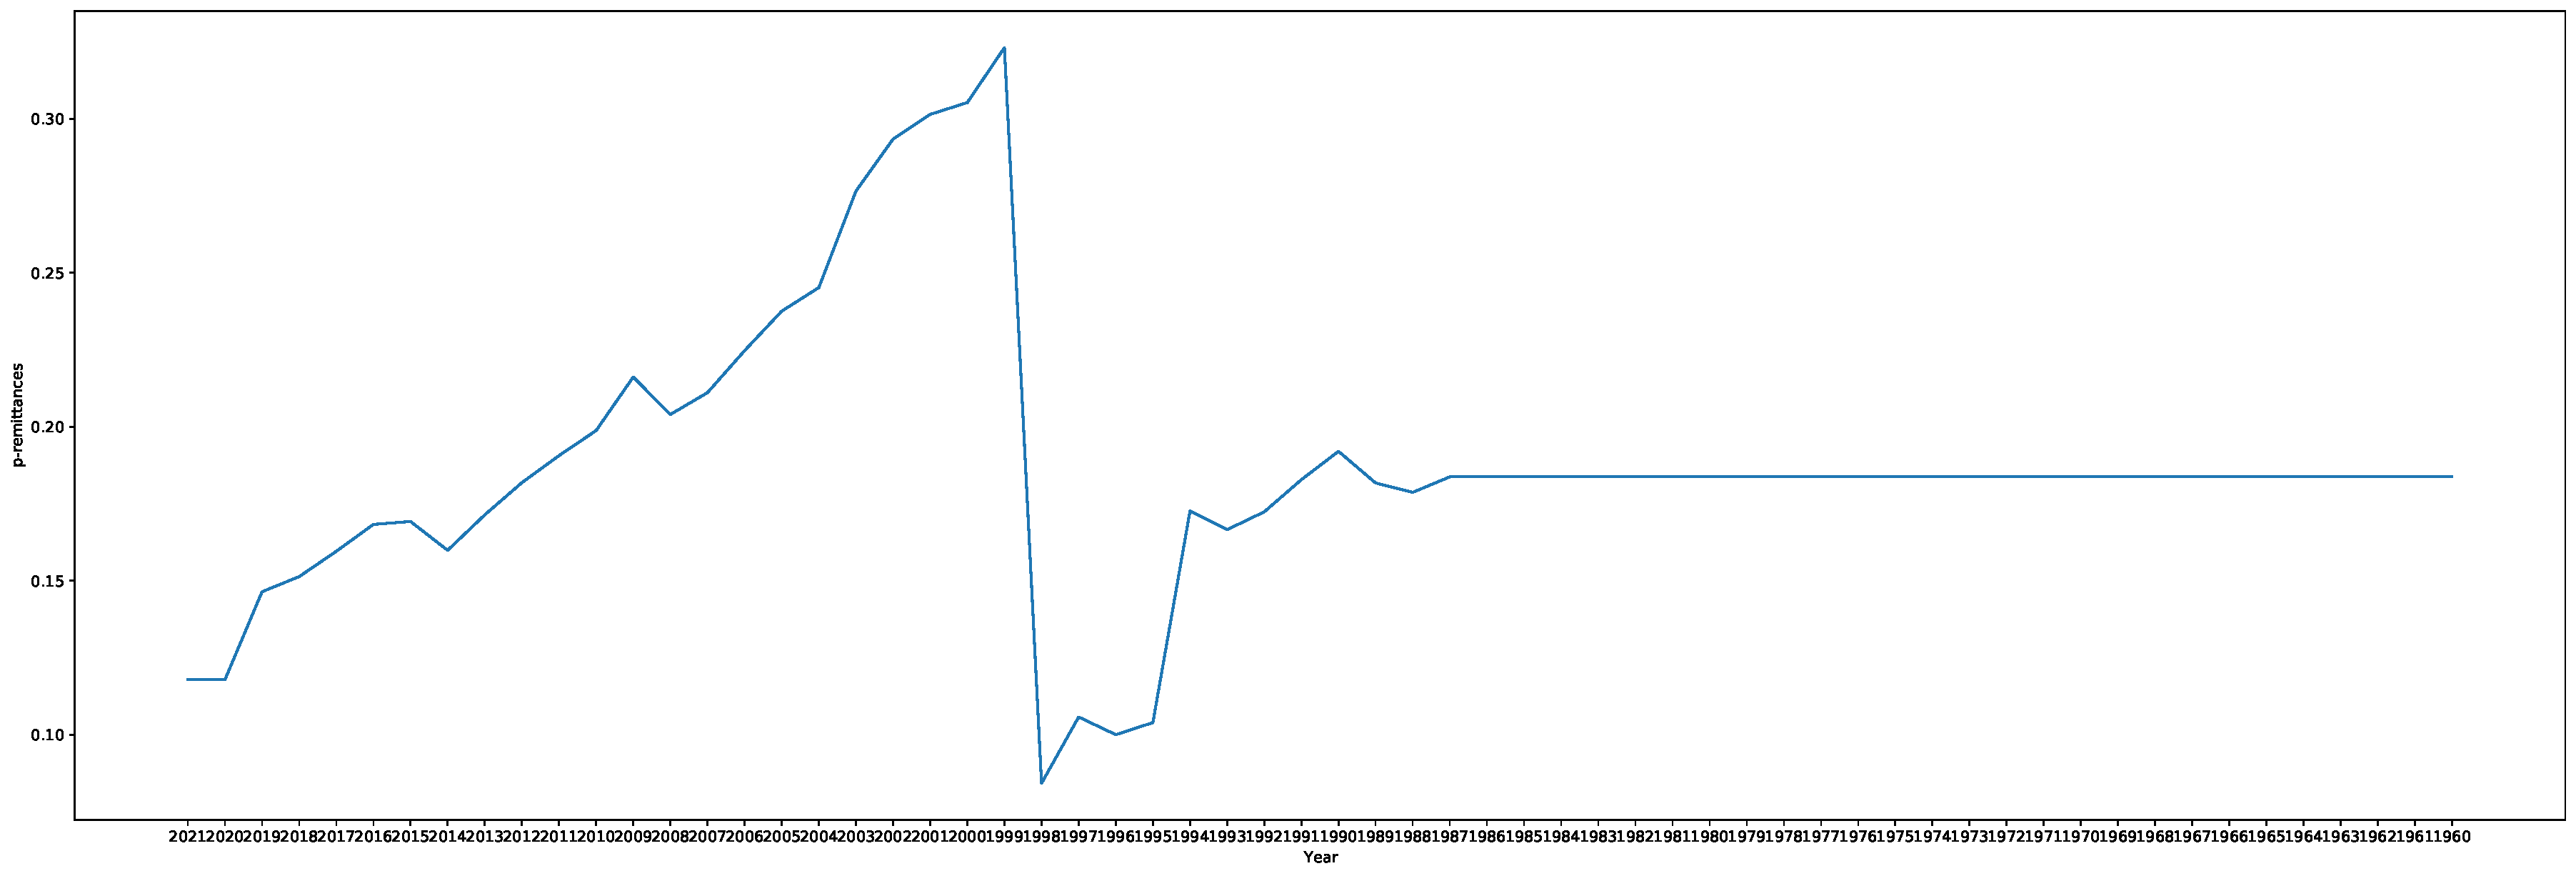
\includegraphics[width=0.7\textwidth]{Images/p-remittances vs year (1).pdf}
    \caption{Personal remittances, received}
    \label{fig1}
\end{figure}

\begin{figure}[H]
    \centering
    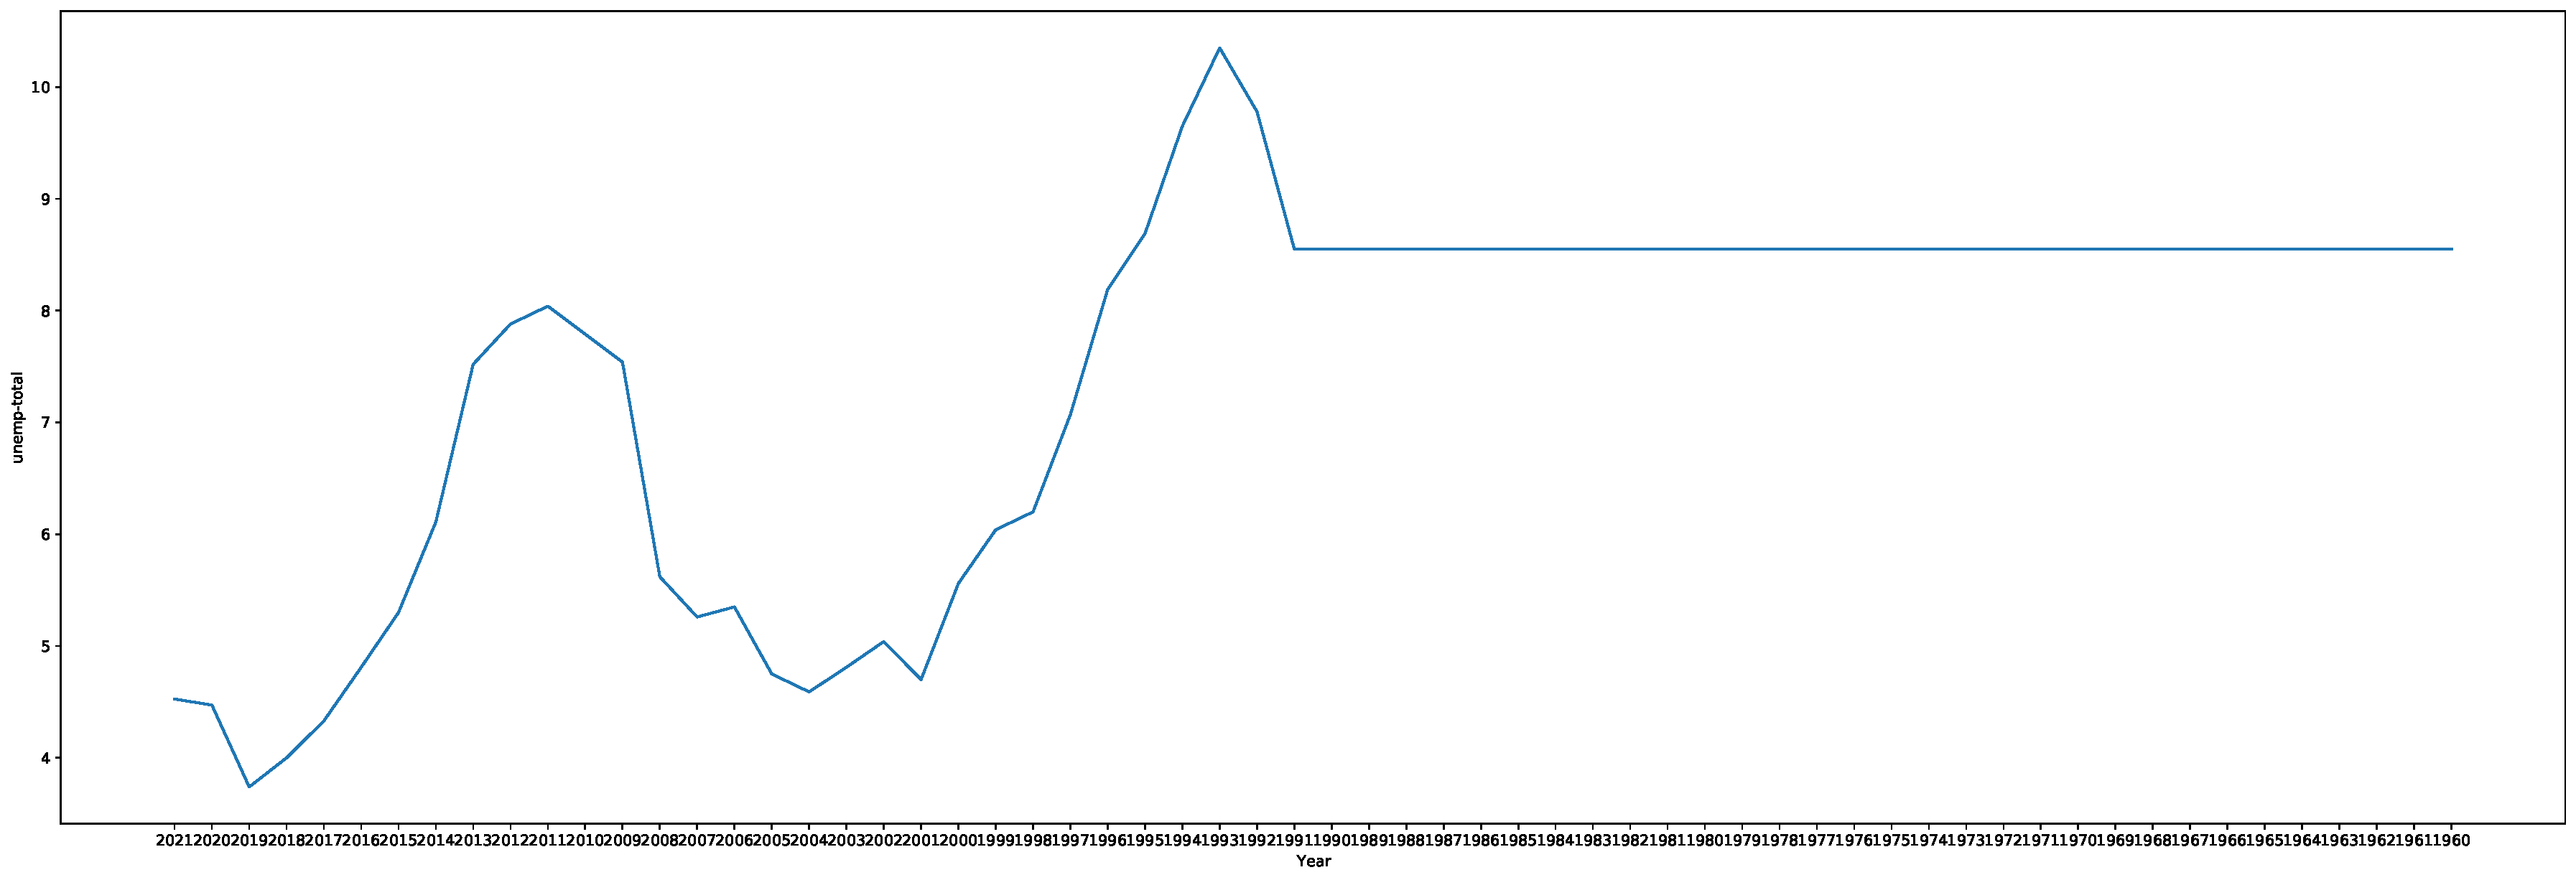
\includegraphics[width=0.7\textwidth]{Images/unemp-total vs year (1).pdf}
    \caption{Unemployment}
    \label{fig1}
\end{figure}

Observation:
\begin{itemize}
  \item Target variable are has rising and falling trend
  \item There is seasonal dips in some years
  \item The target variable is not stationary
\end{itemize}

\vspace{10mm}

\hspace{10mm}\textbf{Basic Information}\\
\begin{figure}[H]
    \centering
    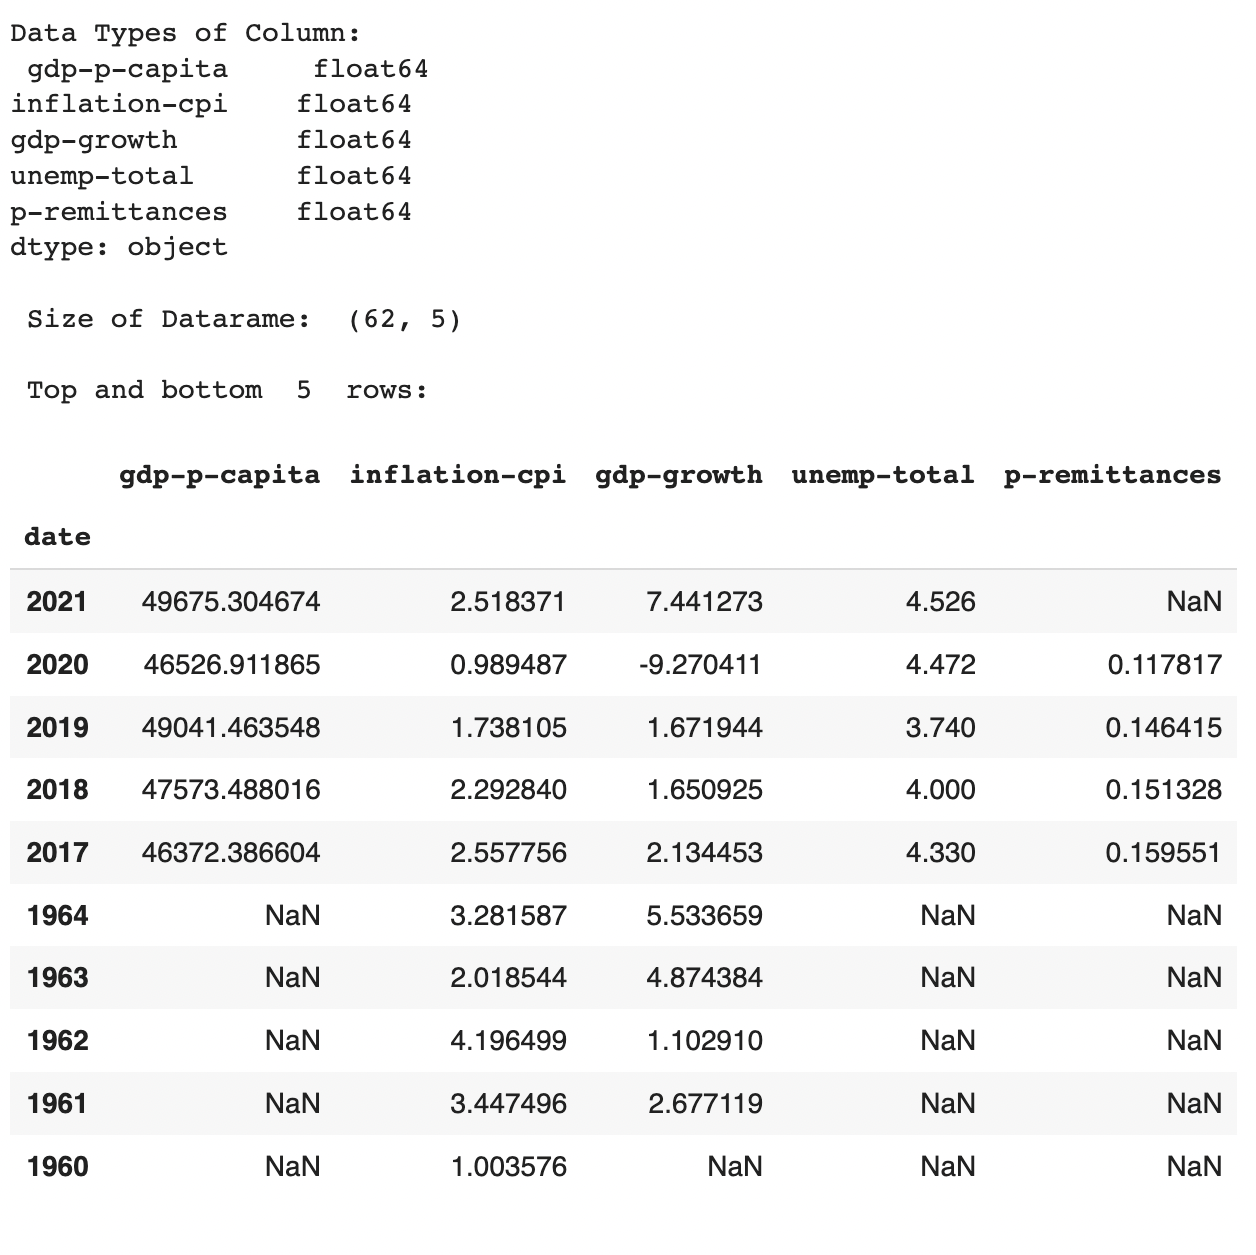
\includegraphics[width=0.7\textwidth]{Images/BasicInfo.png}
\end{figure}

Observation:
\begin{itemize}
 \item head function of pandas library returns first five observation of data and tail function returns last five observation of data
\item info function returns total number of rows and columns of dataset along with data type of each columns. Our dataset had 62 rows and 5 columns. All columns have correct data type.
\end{itemize}

\vspace{10mm}

\begin{tabular}{lrrrrr}
\toprule
{} &  gdp-p-capita &  inflation-cpi &  gdp-growth &  unemp-total &  p-remittances \\
\midrule
count &     62.000000 &      62.000000 &   62.000000 &    62.000000 &      62.000000 \\
mean  &  25148.269450 &       5.048702 &    2.330316 &     7.440452 &       0.186397 \\
std   &  10767.754642 &       4.829198 &    2.603360 &     1.727212 &       0.044724 \\
min   &  17084.598799 &       0.368047 &   -9.270411 &     3.740000 &       0.084190 \\
25\%   &  17084.598799 &       2.117138 &    1.726463 &     5.725000 &       0.174151 \\
50\%   &  17249.095728 &       3.354598 &    2.510750 &     8.550000 &       0.183732 \\
75\%   &  34321.032331 &       5.993608 &    3.630456 &     8.550000 &       0.183732 \\
max   &  49675.304674 &      24.207288 &    7.441273 &    10.350000 &       0.323117 \\
\bottomrule
\end{tabular}
\vspace{10mm}


Observation:
\begin{itemize}
    \item Mean value is greater than median value represented by 50th percentile for some columns
\item There is big difference between 75th percentile and max value for columns like inflation-cpi,gdp-growth,unemp-total
\item The above points hints might be there is outliers present in data set. Let's look into histograms to get some conclusion.
\end{itemize}


\begin{figure}[H]
    \centering
    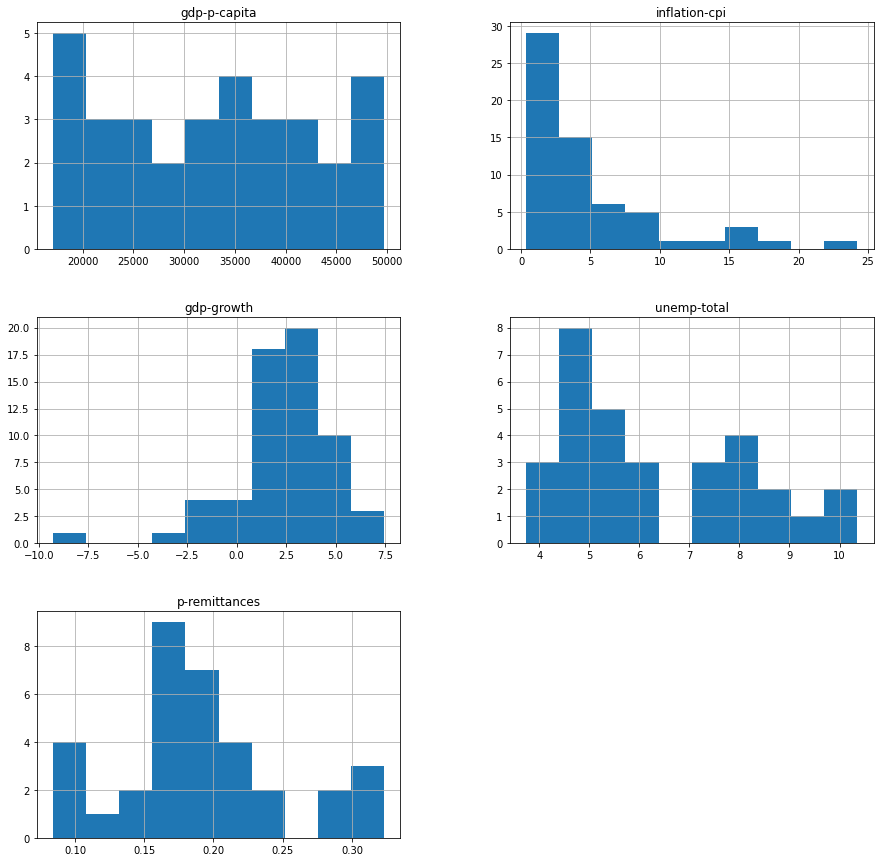
\includegraphics[width=0.7\textwidth]{Images/histograms.png}
    \caption{Data Histograms}
    \label{fig1}
\end{figure}

\vspace{10mm}

\hspace{10mm}\textbf{Missing Values Handling}\\

\begin{figure}[H]
    \centering
    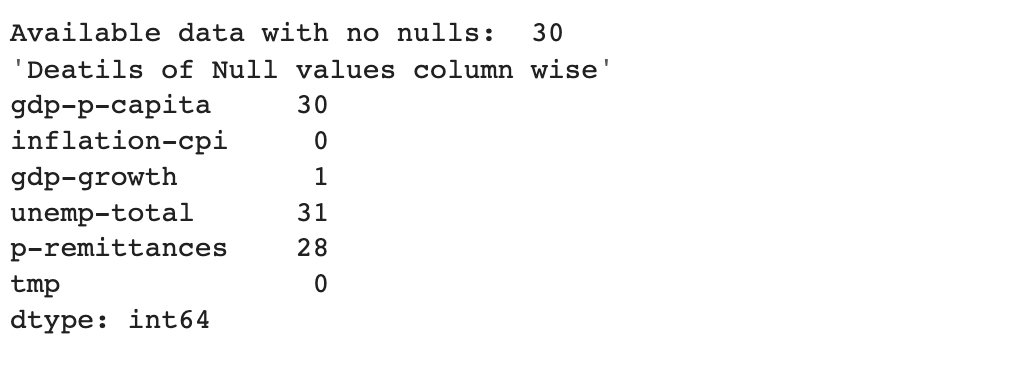
\includegraphics[width=0.7\textwidth]{Images/Missing.png}
\end{figure}

Observation:
\begin{itemize}
    \item We can see we have lot of missing value in columns
\item Action needed to handle this missing data
\end{itemize}

\vspace{30mm}

\begin{lstlisting}[language=Python]
# This function fill missing values
def fill_miss(d_f,metd = None):
    col_name = d_f.columns
    av_method = ['bfill', 'pad', 'ffill', 'linear','mean']

    if metd == None:
        return d_f
    for col in col_name:    
      if (metd == 'mean'):
          d_f[col] = d_f[col].fillna(value=d_f[col].mean()) 
      elif metd == 'linear':
          d_f[col] = d_f[col].interpolate(method = 'linear') 
      elif  metd in av_method:
          d_f[col] = d_f[col].fillna(method = metd)
      else:
          print("Invalid fill type")
          return d_f

fill_miss(df2, 'ffill')
fill_miss(df2, 'bfill')
missing_value(df2) 

\end{lstlisting}

\begin{figure}[H]
    \centering
    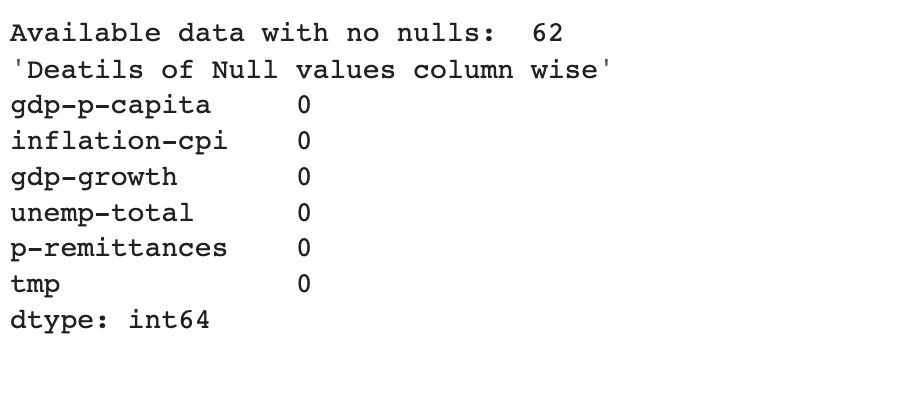
\includegraphics[width=0.7\textwidth]{Images/fixed_missing.png}
\end{figure}

Observation:
\begin{itemize}
    \item We can see now there is no missing value in our data
\item We used Next Observation Carried Forward and Last Observation carried Forward to fill our missing data
\item We are ready for further processing of data
\end{itemize}

\vspace{50mm}

\hspace{10mm}\textbf{Outlier detection and corrections}\\

\begin{lstlisting}[language=Python]
# Outlier Detection using Inter Quartile Range
def out_iqr(s, k=1.5, return_thresholds=False):
    """
    Return a boolean mask of outliers for a series
    using interquartile range, works column-wise.
    param k:
        some cutoff to multiply by the iqr
    :type k: ``float``
    param return_thresholds:
        True returns the lower and upper bounds, good for plotting.
        False returns the masked array 
    :type return_thresholds: ``bool``
    """
    # calculate interquartile range
    q25, q75 = np.percentile(s, 25), np.percentile(s, 75)
    iqr = q75 - q25
    # calculate the outlier cutoff
    cut_off = iqr * k
    lower, upper = q25 - cut_off, q75 + cut_off
    if return_thresholds:
        return lower, upper
    else: # identify outliers
        return [True if x < lower or x > upper else False for x in s]
    
    
# For comparison, make one array each at varying values of k.
df3 = df2.drop(columns=['tmp'],axis=1)
iqr1 = df3.apply(out_iqr, k=1.5)
iqr1.head(10)
\end{lstlisting}

\begin{tabular}{llllll}
\toprule
{} &  gdp-p-capita &  inflation-cpi &  gdp-growth &  unemp-total &  p-remittances \\
date &               &                &             &              &                \\
\midrule
2021 &         False &          False &        True &        False &           True \\
2020 &         False &          False &        True &        False &           True \\
2019 &         False &          False &       False &        False &           True \\
2018 &         False &          False &       False &        False &           True \\
2017 &         False &          False &       False &        False &           True \\
2016 &         False &          False &       False &        False &          False \\
2015 &         False &          False &       False &        False &          False \\
2014 &         False &          False &       False &        False &          False \\
2013 &         False &          False &       False &        False &          False \\
2012 &         False &          False &       False &        False &          False \\
\bottomrule
\end{tabular}

\vspace{2mm}
Observation:
\begin{itemize}
    \item Above table is first 10 row of data set 'True' represents outliers.
    \item The Interquartile range (IQR) is calculated as the difference between the 75th and the 25th percentiles of the data. The IQR can be used to identify outliers by defining limits on the sample values that are a factor k of the IQR below the 25th percentile or above the 75th percentile. The common value for the factor k is the value 1.5 (which we have used here). A factor k of 3 or more can be used to identify values that are extreme outliers or far outs.
    \item We replaced all outliers with Nan value used linear interpolation Nan values( code can be found in above python script).
    
\end{itemize}

\begin{tabular}{lrrrrr}
\toprule
{} &  gdp-p-capita &  inflation-cpi &  gdp-growth &  unemp-total &  p-remittances \\
date &               &                &             &              &                \\
\midrule
2021 &  49675.304674 &       2.518371 &    7.441273 &        4.526 &       0.117817 \\
2020 &  46526.911865 &       0.989487 &   -9.270411 &        4.472 &       0.117817 \\
2019 &  49041.463548 &       1.738105 &    1.671944 &        3.740 &       0.146415 \\
2018 &  47573.488016 &       2.292840 &    1.650925 &        4.000 &       0.151328 \\
2017 &  46372.386604 &       2.557756 &    2.134453 &        4.330 &       0.159551 \\
\bottomrule
\end{tabular}

\vspace{10mm}

\begin{figure}[H]
    \centering
    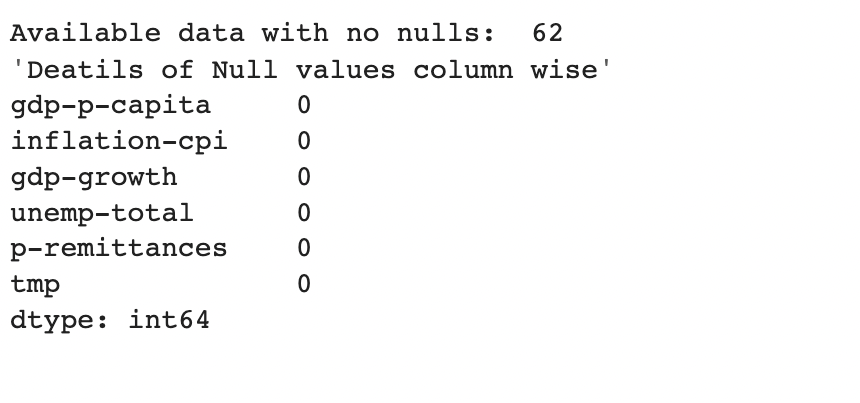
\includegraphics[width=0.7\textwidth]{Images/outlier_fix.png}
\end{figure}

Observations: As we can see in above table and image there no outliers in data set.


\vspace{50mm}

\subsection{EDA: Inspection, Data Profiling, Visualisation and Making Data Stationary  }

\textbf{Seasonally Decomposition of Data}\\

\begin{figure}[H]
    \centering
    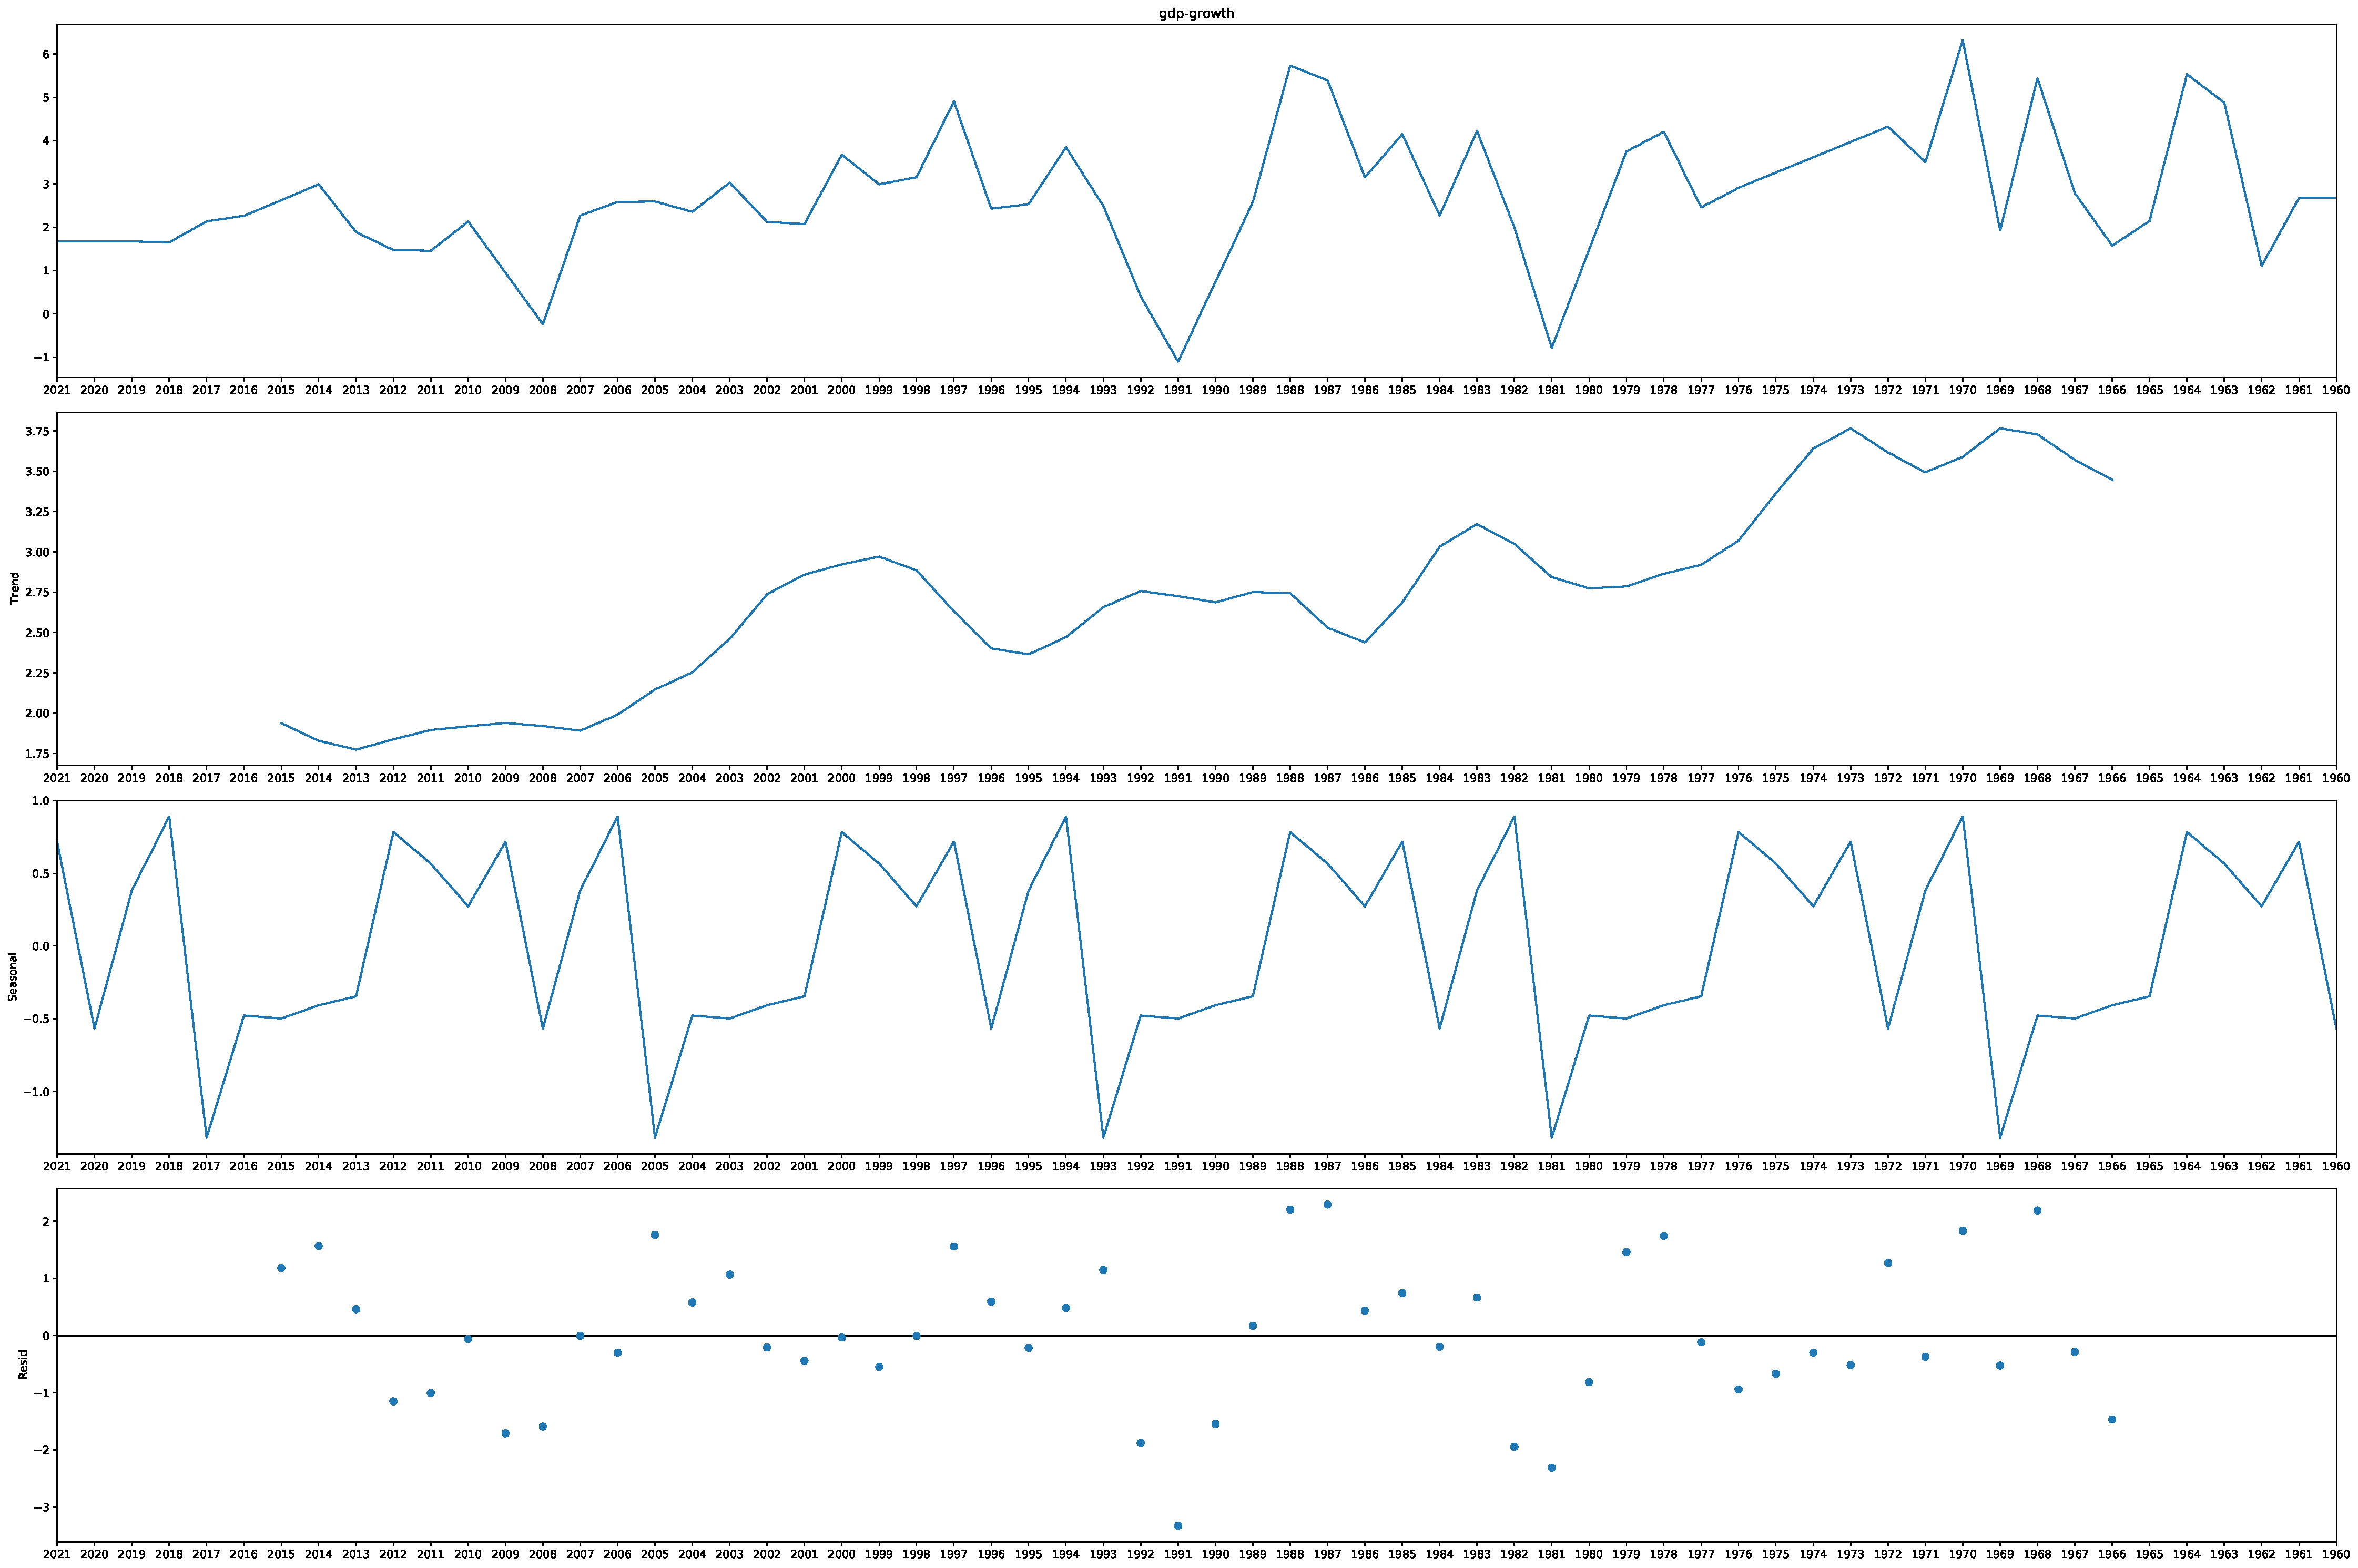
\includegraphics[width=0.7\textwidth]{Images/gdp-growth_decompose.pdf}
    \caption{GDP Growth}
    \label{fig1}
\end{figure}

\begin{figure}[H]
    \centering
    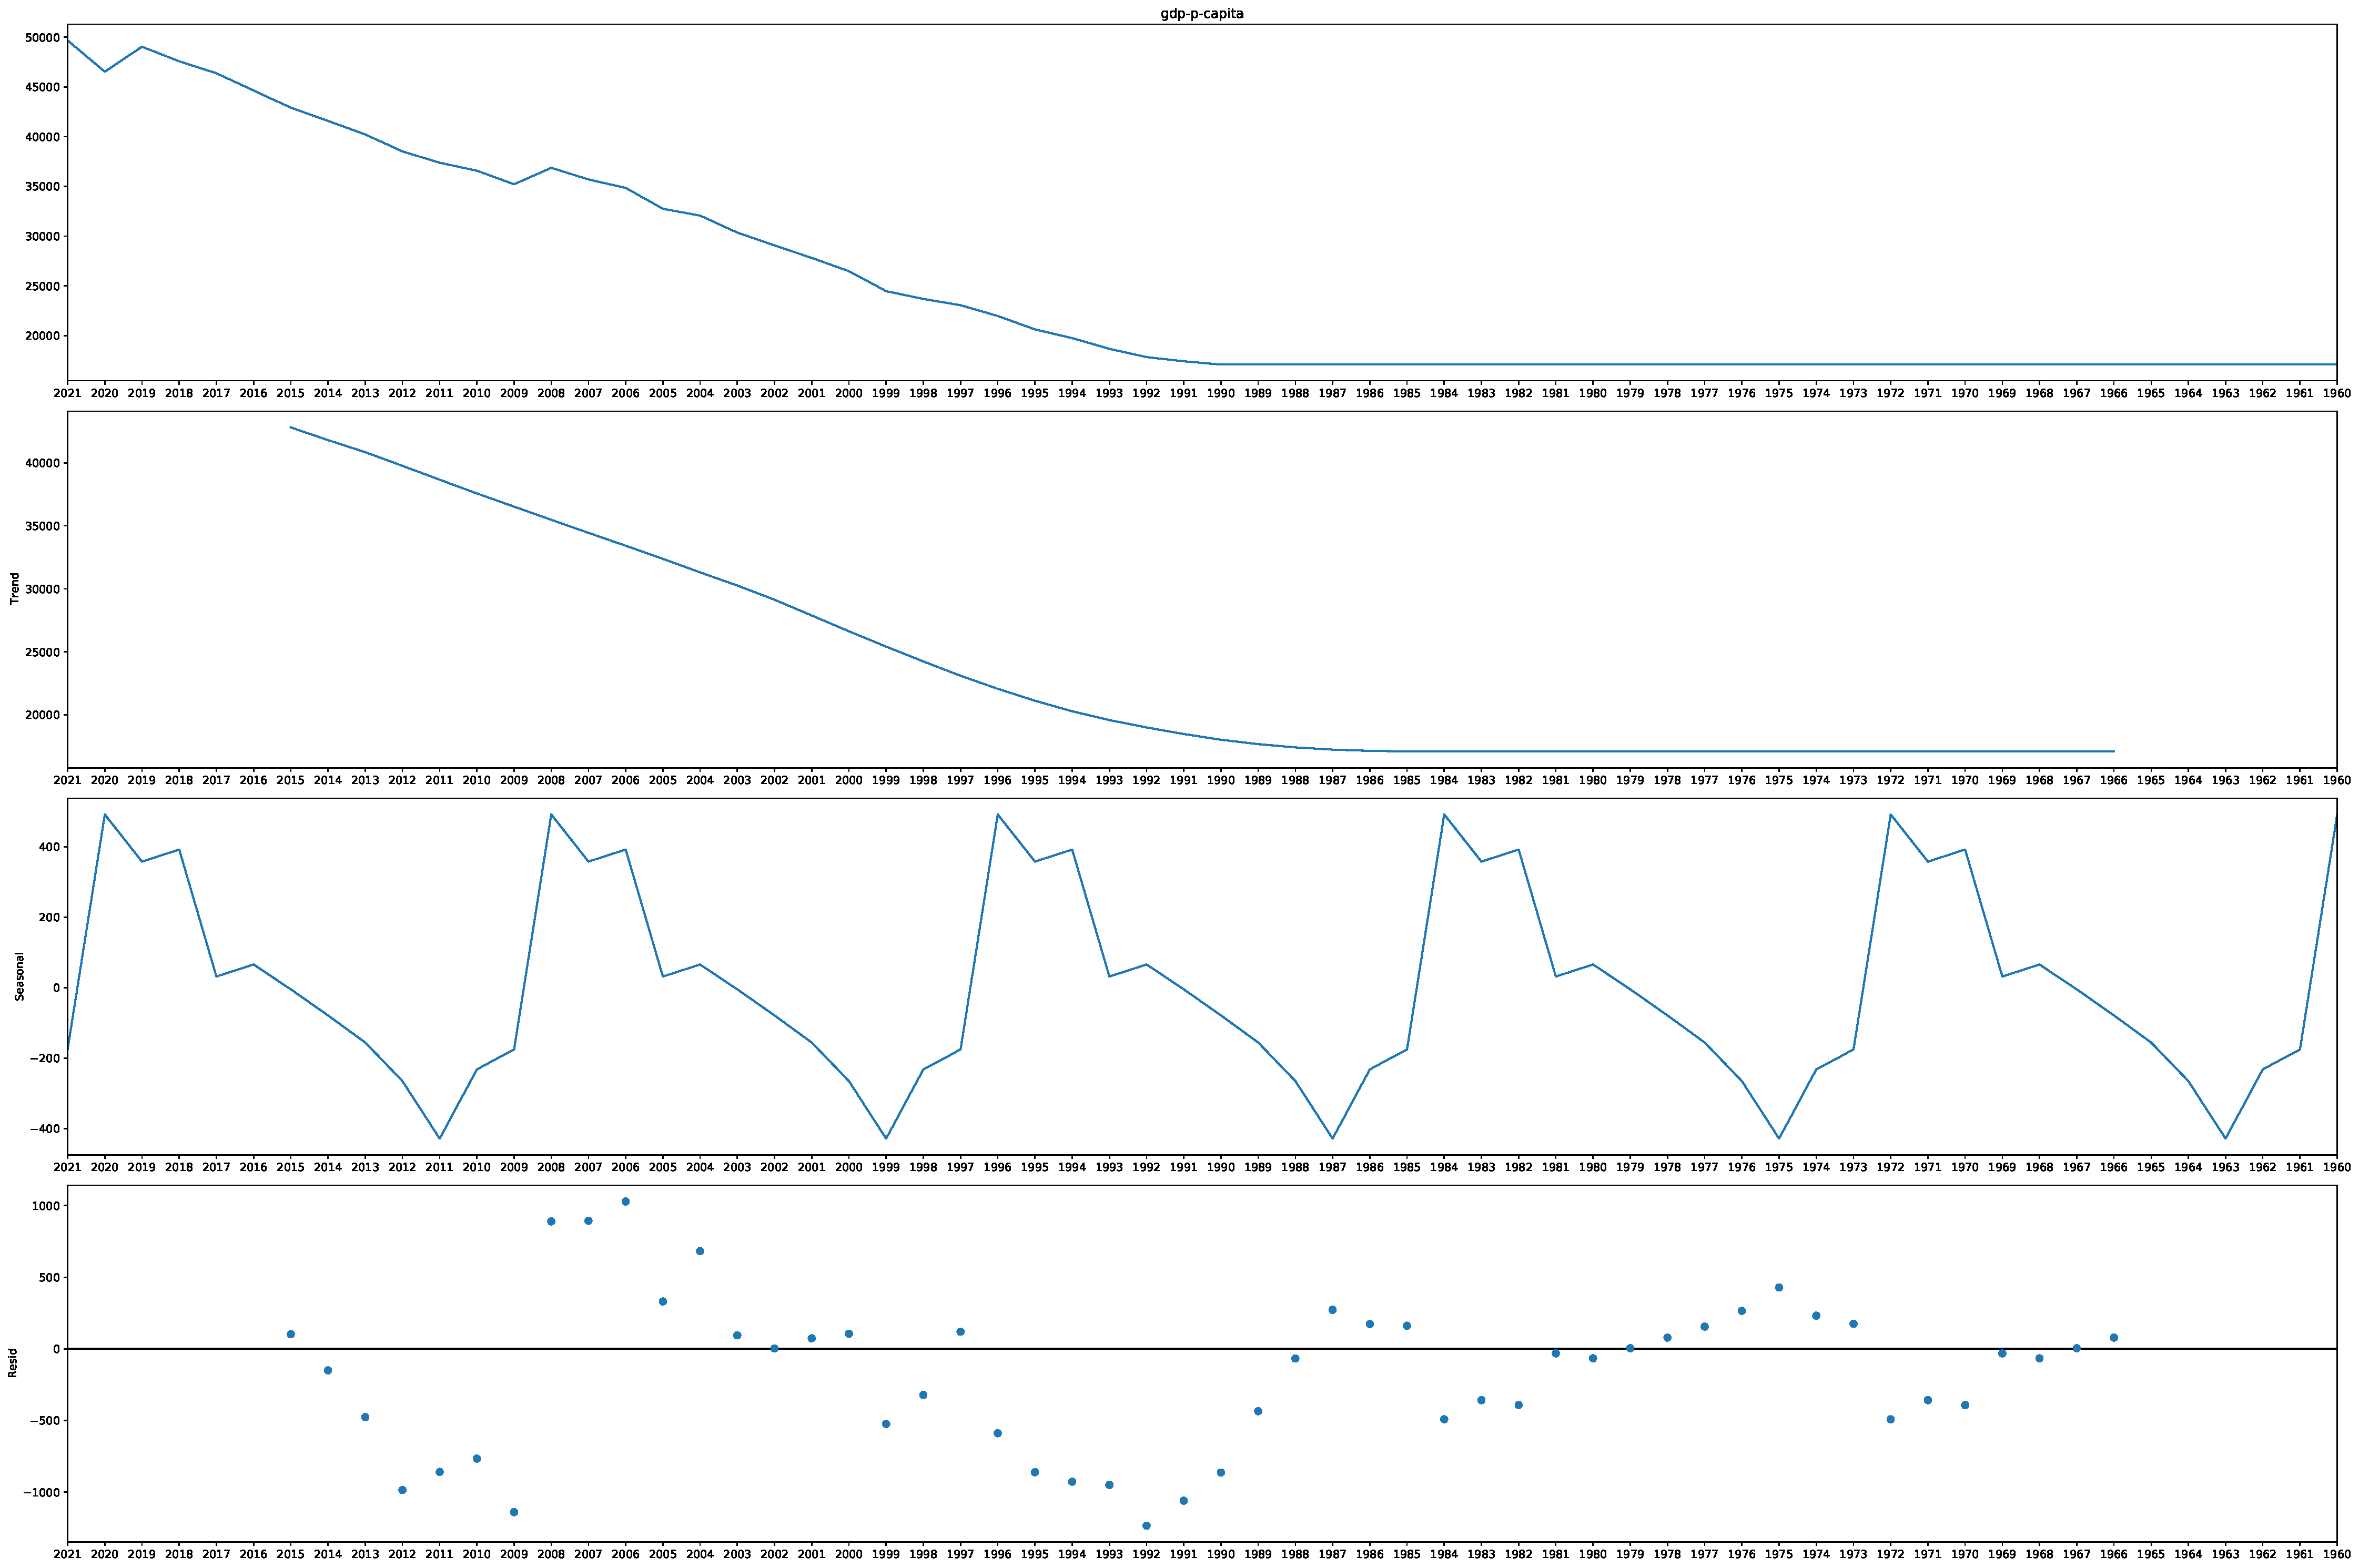
\includegraphics[width=0.7\textwidth]{Images/gdp-p-capita_decompose.pdf}
    \caption{GDP Person Capita}
    \label{fig1}
\end{figure}


\begin{figure}[H]
    \centering
    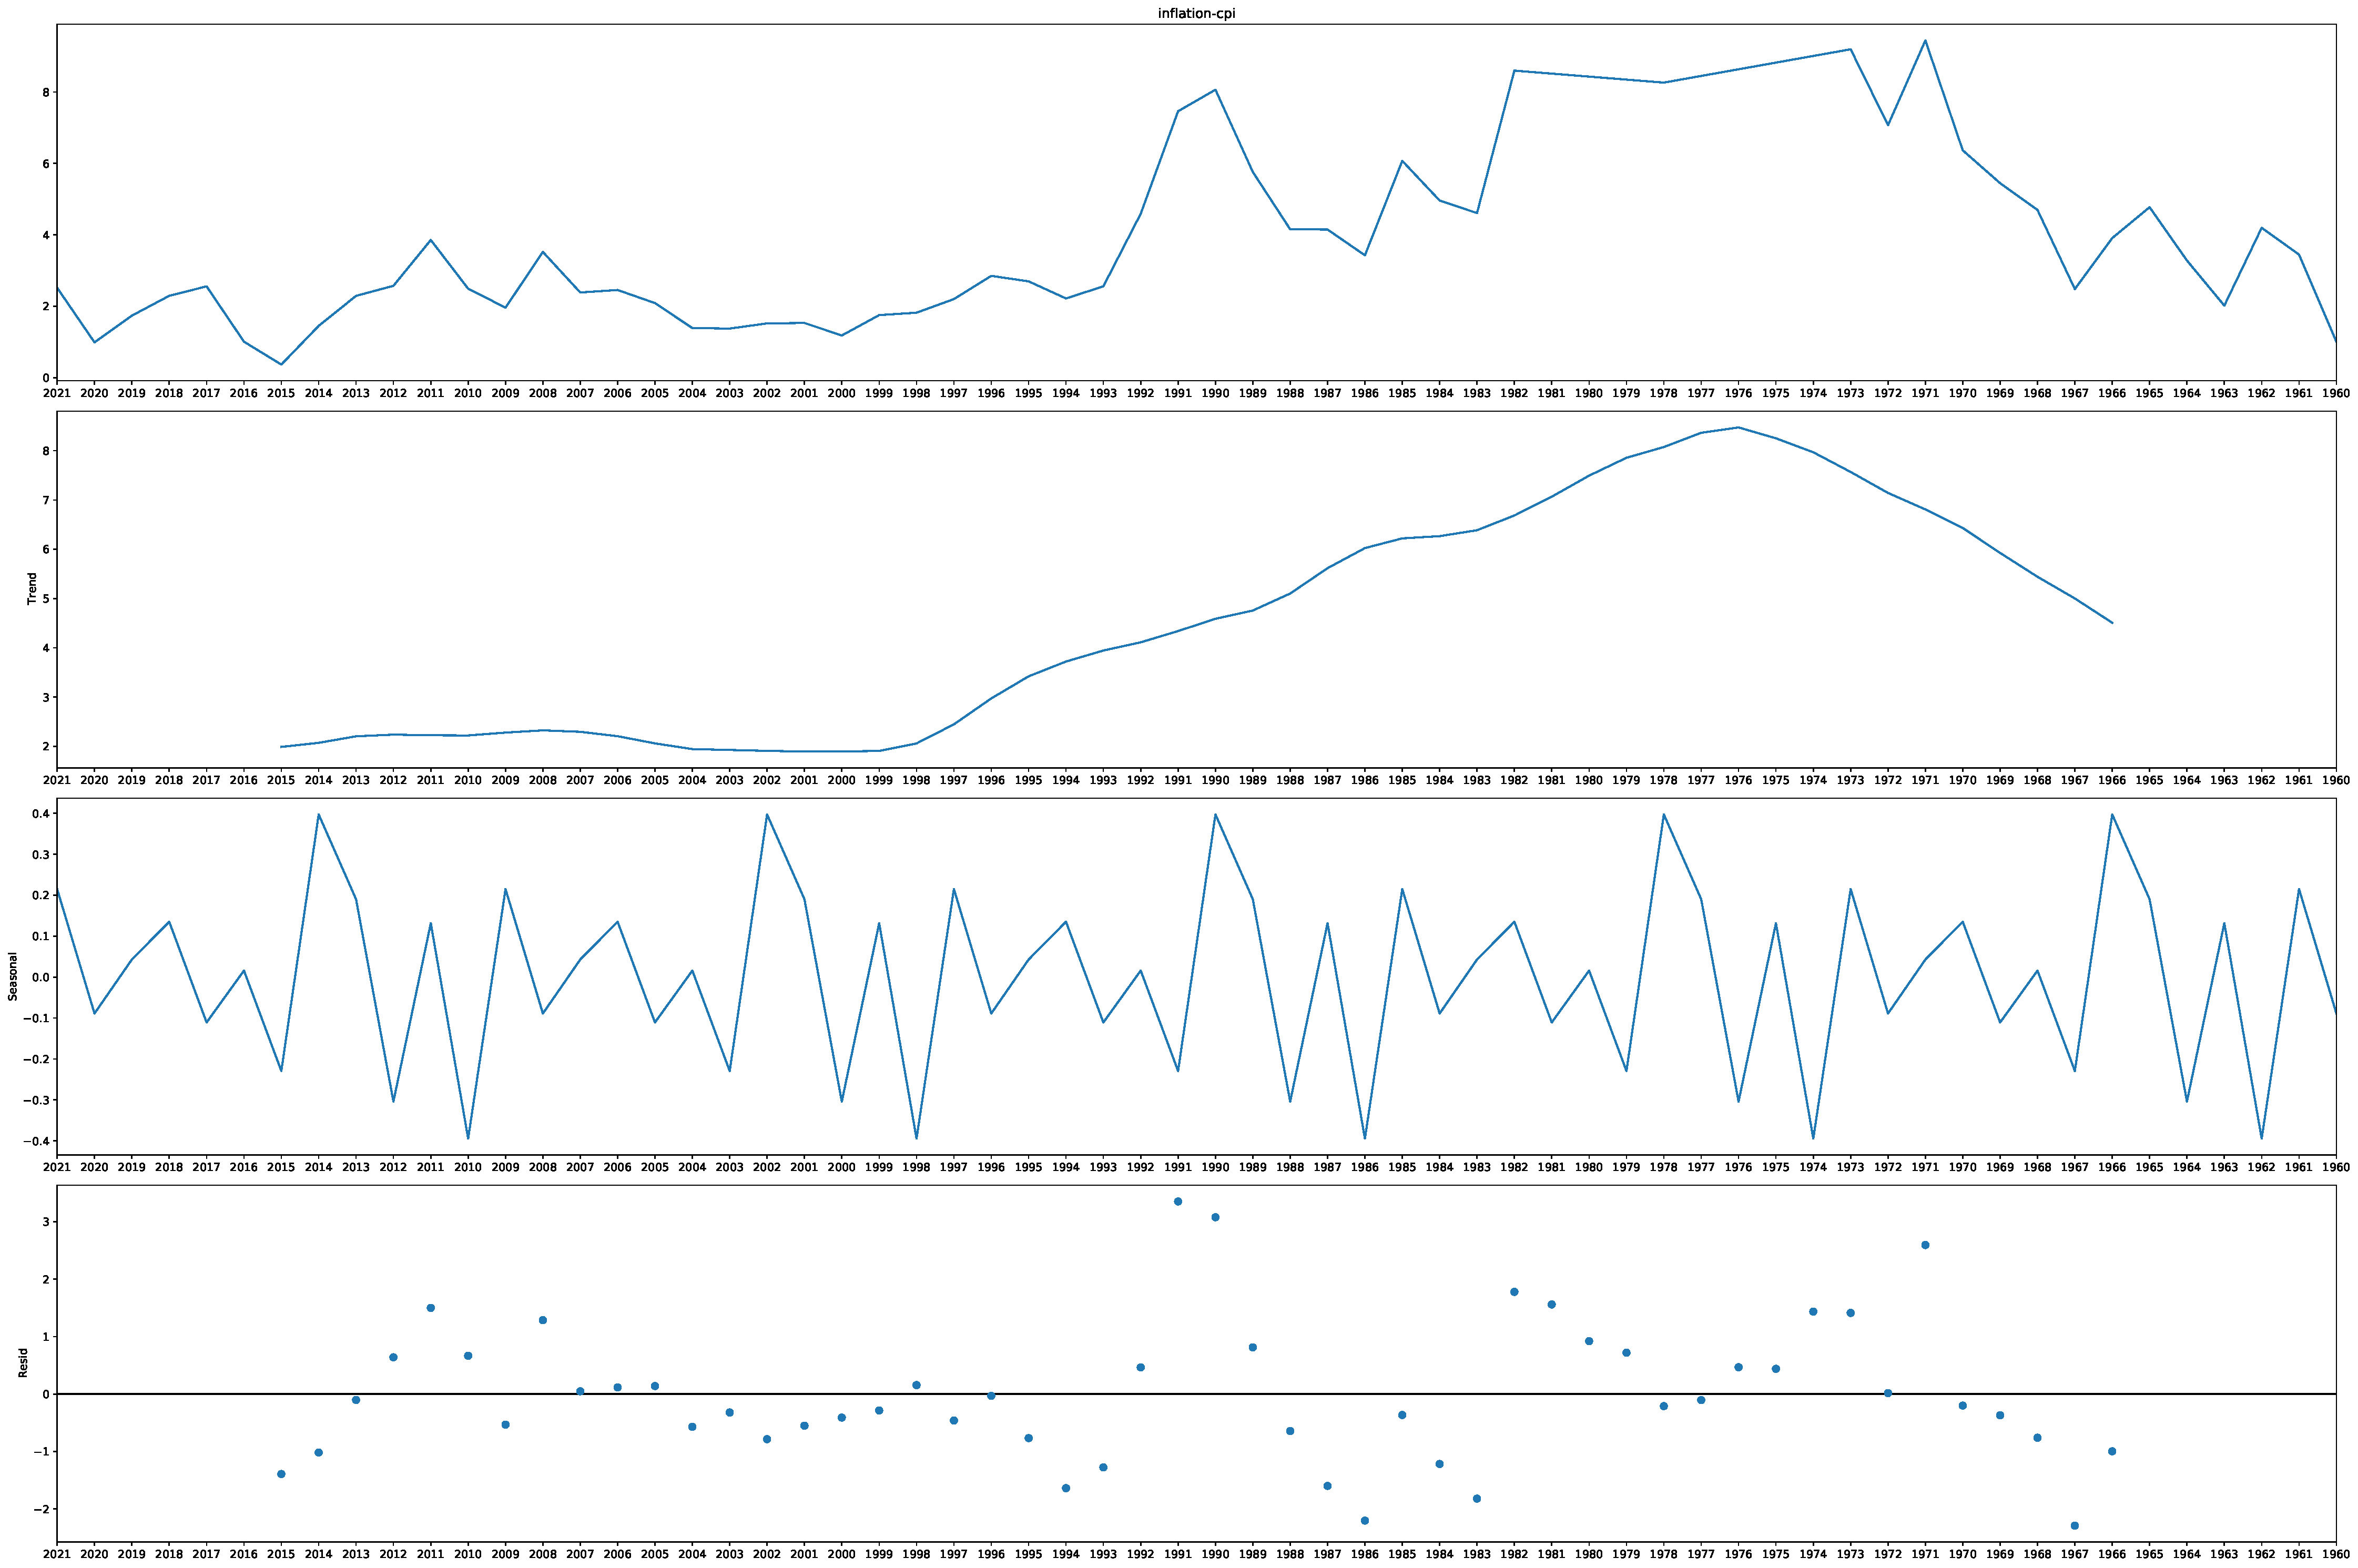
\includegraphics[width=0.7\textwidth]{Images/inflation-cpi_decompose.pdf}
    \caption{Inflation}
    \label{fig1}
\end{figure}


\begin{figure}[H]
    \centering
    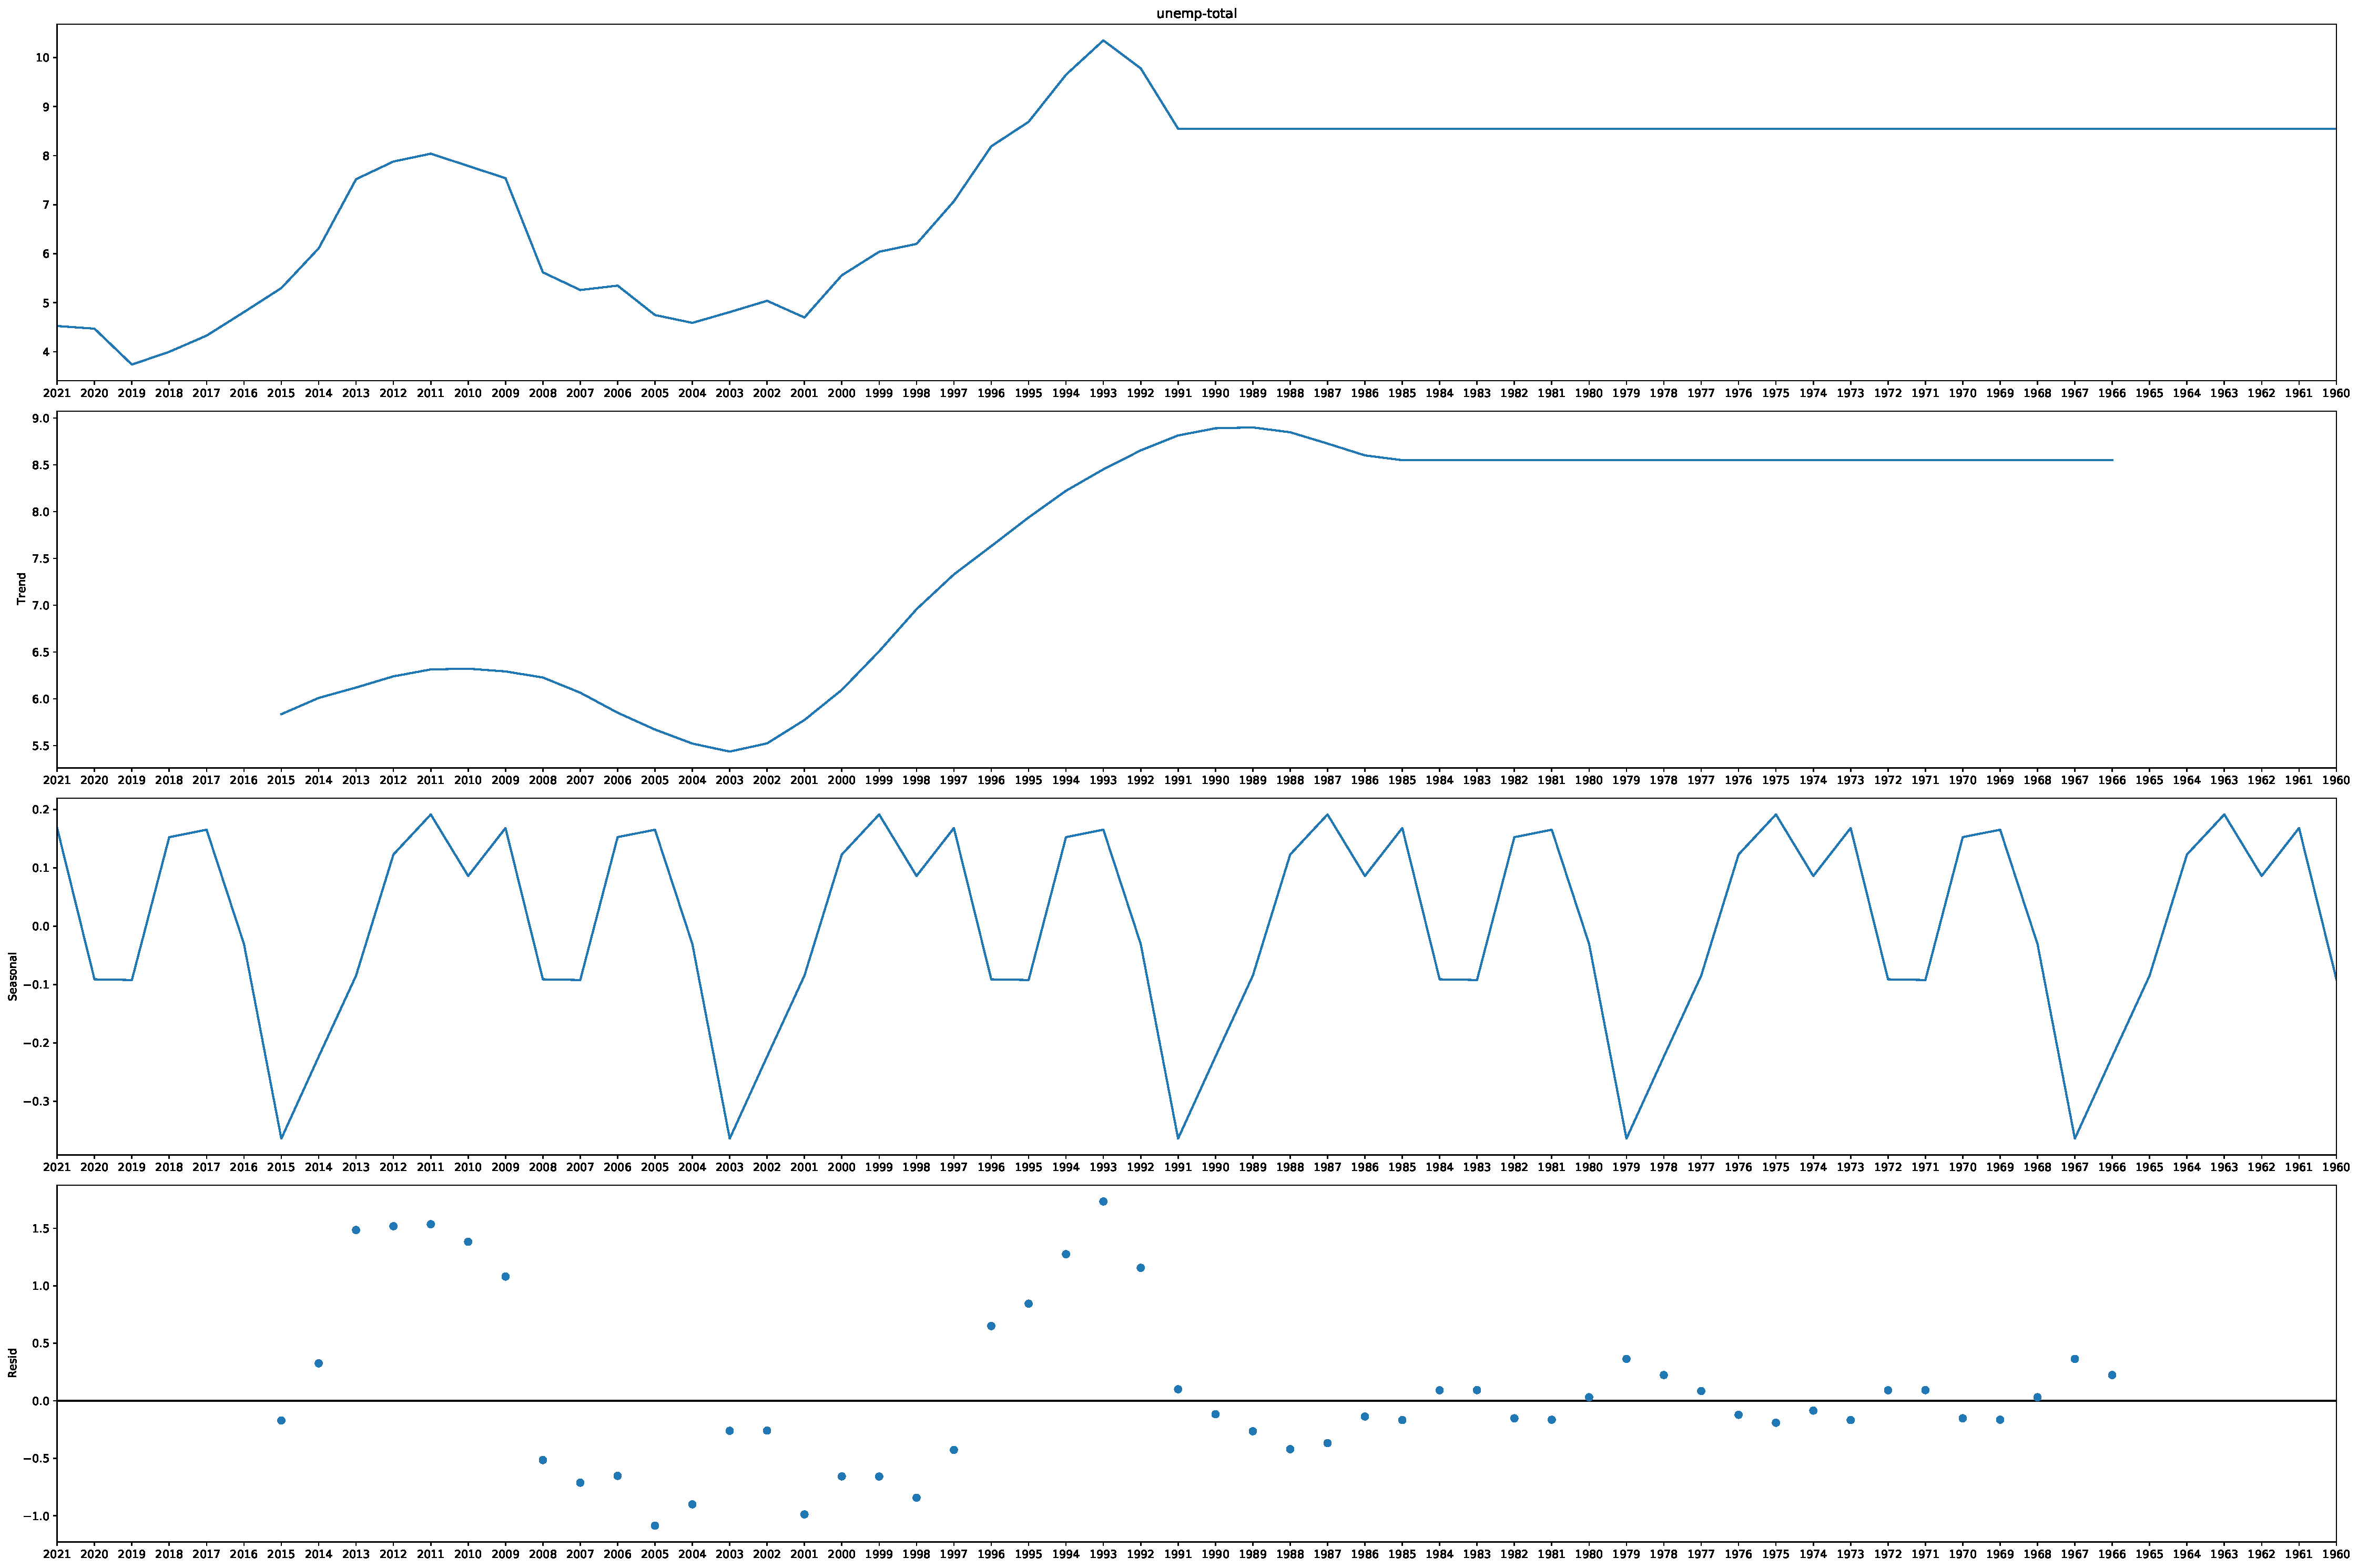
\includegraphics[width=0.7\textwidth]{Images/unemp-total_decompose.pdf}
    \caption{Unemployment}
    \label{fig1}
\end{figure}

Observation:
\begin{itemize}
    \item We use additive model for decomposition of our data as time series data consists of Time Series Data = Trend + Seasonal + Random .
\item We can observe that trend is having slope and seasonal pattern is regularly repeating pattern kind of.
\end{itemize}

\vspace{20mm}
\textbf{Auto-correlation and Partial Auto-correlation Graphs}\\
\begin{figure}[H]
    \centering
    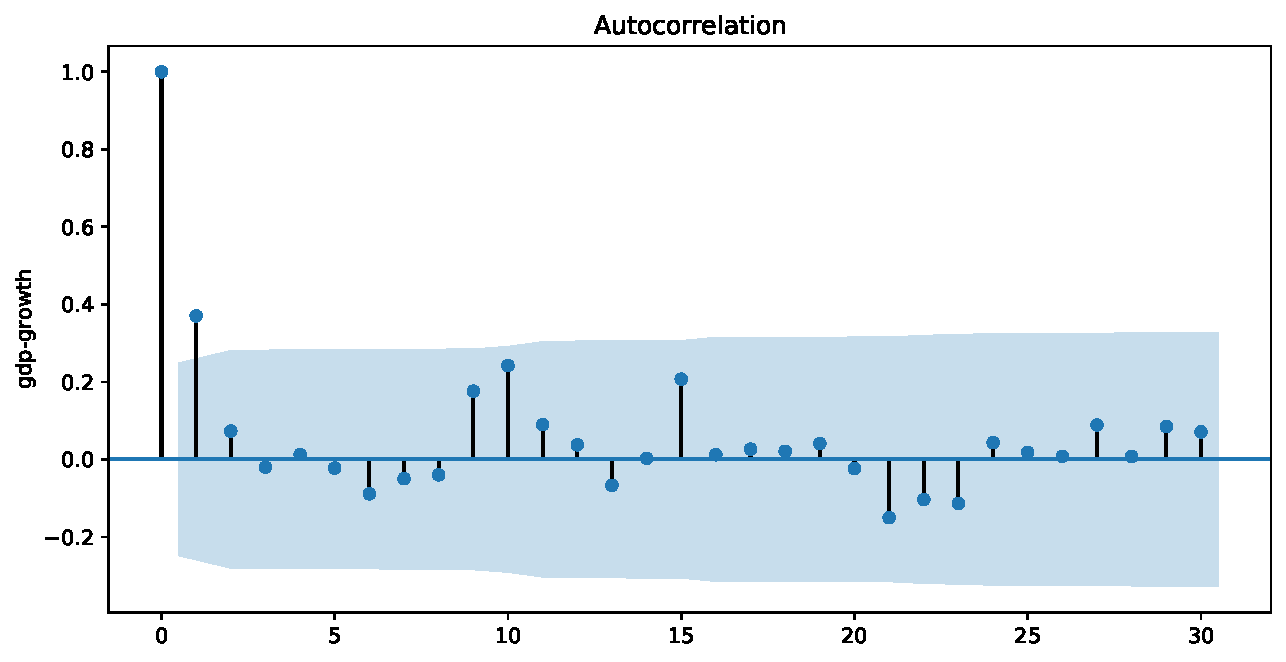
\includegraphics[width=0.7\textwidth]{Images/gdp-growth_Acorr.pdf}
    \caption{GDP Growth}
    \label{fig1}
\end{figure}

\begin{figure}[H]
    \centering
    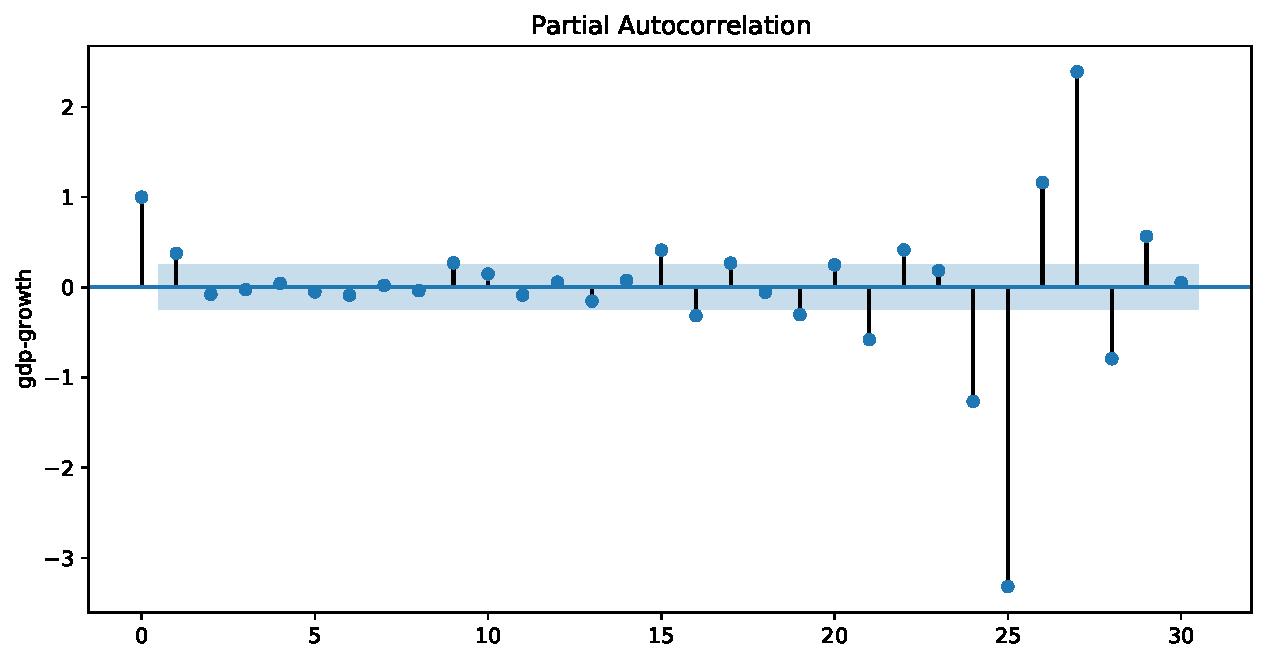
\includegraphics[width=0.7\textwidth]{Images/gdp-growth_PAcorr.pdf}
    \caption{GDP Growth}
    \label{fig1}
\end{figure}

\begin{figure}[H]
    \centering
    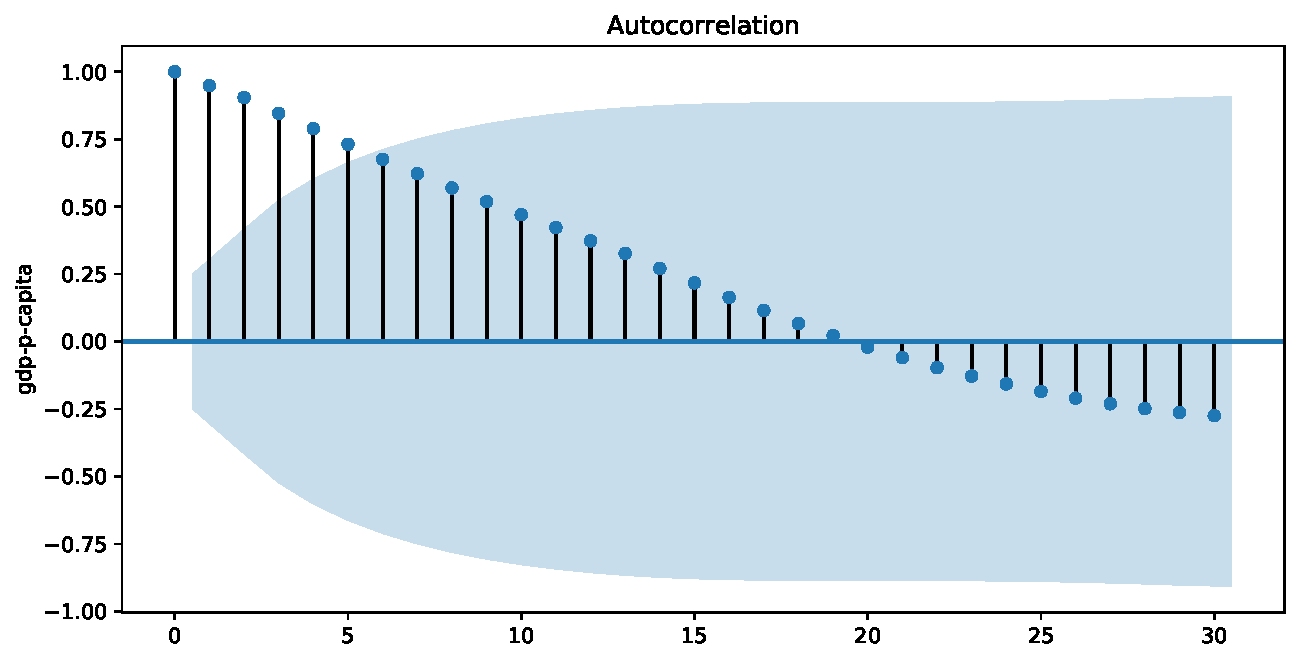
\includegraphics[width=0.7\textwidth]{Images/gdp-p-capita_Acorr.pdf}
    \caption{GDP Person Capita}
    \label{fig1}
\end{figure}

\begin{figure}[H]
    \centering
    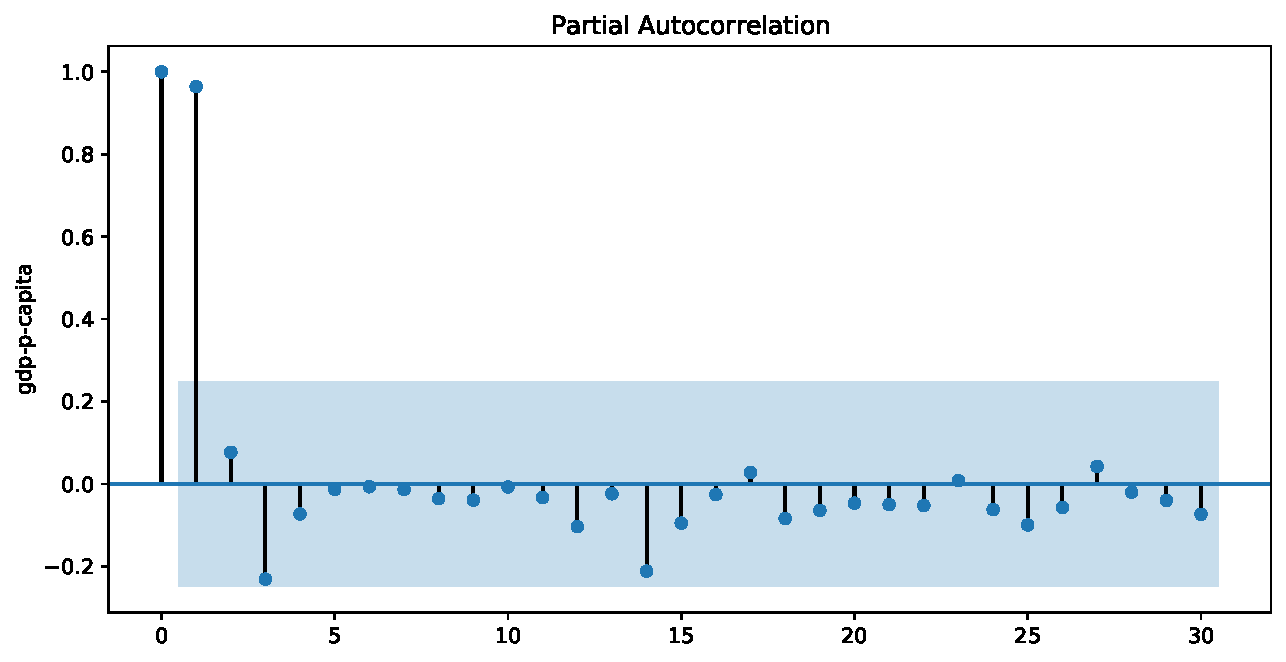
\includegraphics[width=0.7\textwidth]{Images/gdp-p-capita_PAcorr.pdf}
    \caption{GDP Person Capita}
    \label{fig1}
\end{figure}


\begin{figure}[H]
    \centering
    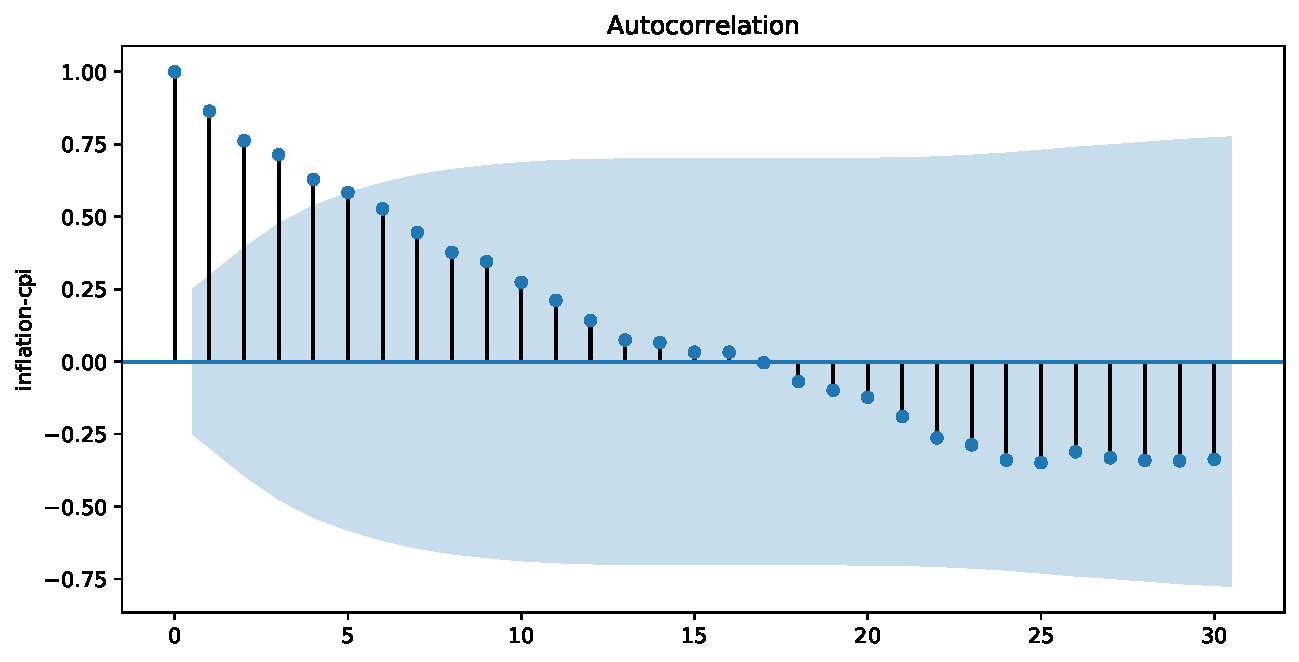
\includegraphics[width=0.7\textwidth]{Images/inflation-cpi_Acorr.pdf}
    \caption{Inflation}
    \label{fig1}
\end{figure}


\begin{figure}[H]
    \centering
    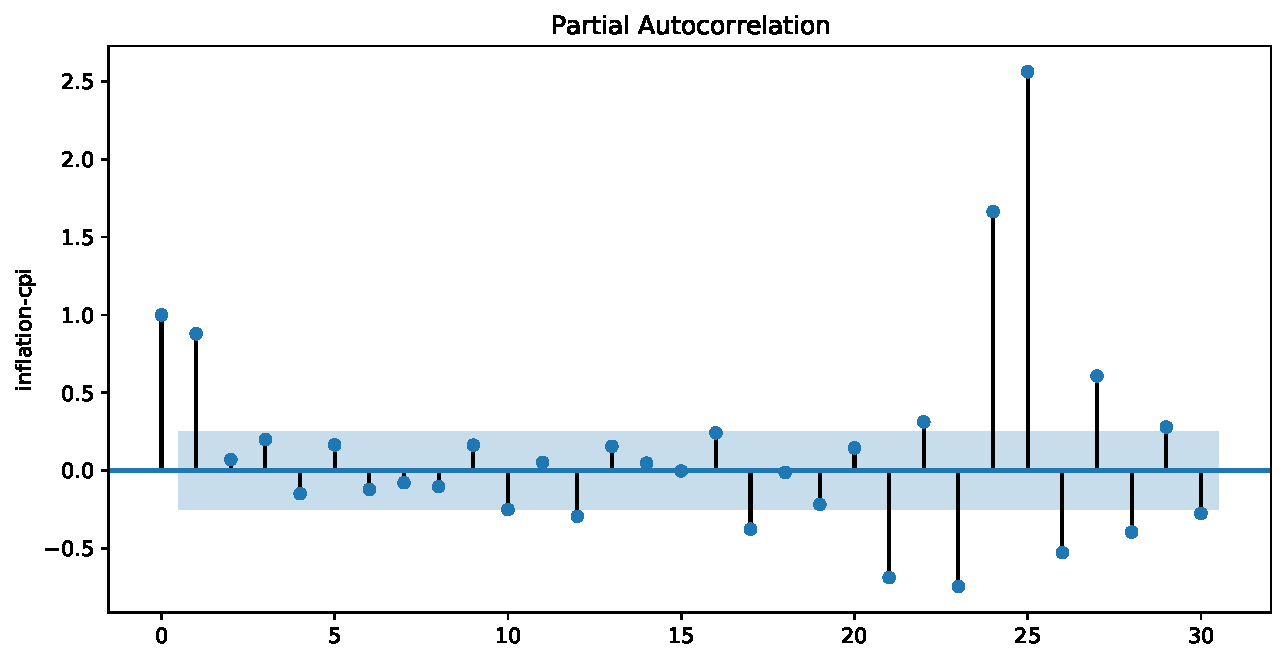
\includegraphics[width=0.7\textwidth]{Images/inflation-cpi_PAcorr.pdf}
    \caption{Inflation}
    \label{fig1}
\end{figure}

\begin{figure}[H]
    \centering
    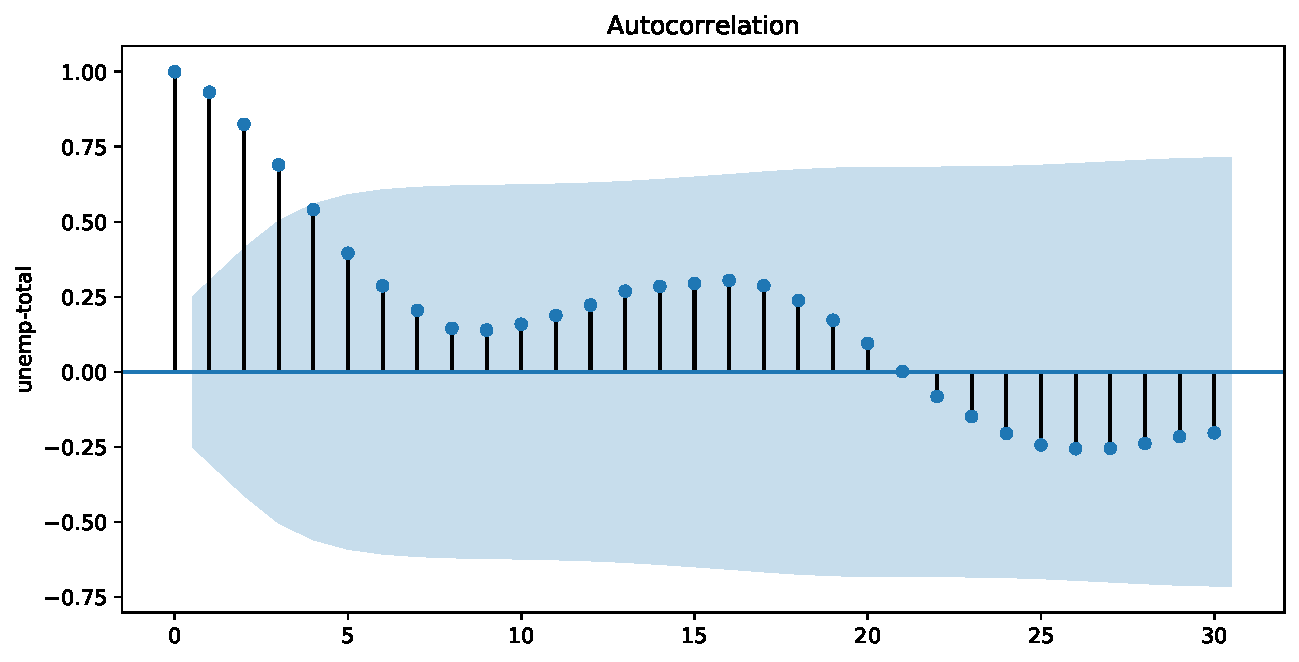
\includegraphics[width=0.7\textwidth]{Images/unemp-total_Acorr.pdf}
    \caption{Unemployment}
    \label{fig1}
\end{figure}

\begin{figure}[H]
    \centering
    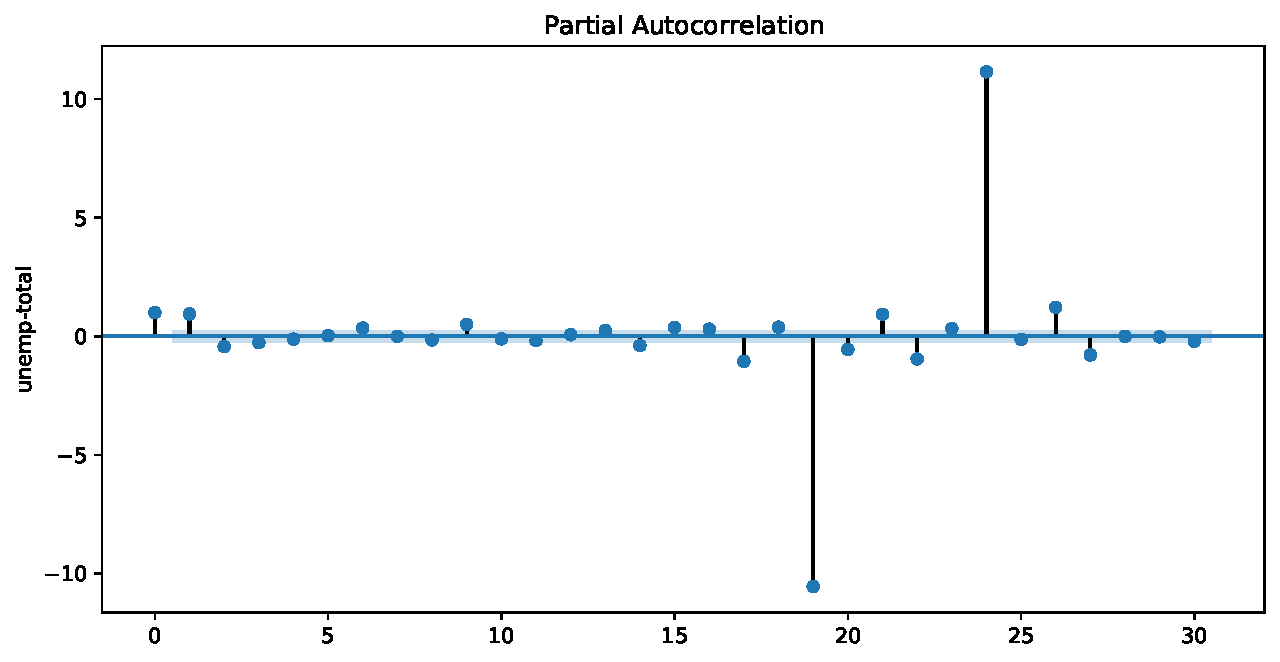
\includegraphics[width=0.7\textwidth]{Images/unemp-total_PAcorr.pdf}
    \caption{Unemployment}
    \label{fig1}
\end{figure}

Observation: There some columns are non-stationary can be seen from the ACF and PACF

\vspace{10mm}
\textbf{Script: for checking stationary and making stationary}\\
\begin{lstlisting}[language=Python]
## Testing statinarity using Agumented Dicky Fuler Unit Root Test
level = []
from statsmodels.tsa.stattools import adfuller
for (columnName, columnData) in df4.iteritems():
    if columnName != 'tmp':
      print('Series:',columnName)
      X = columnData.dropna().values
      result = adfuller(X)
      print('ADF Statistic: %f' % result[0])
      print('p-value: %f' % result[1])
      print('Critical Values:')
      for key, value in result[4].items():
          print('\t%s: %.3f' % (key, value))
      if (result[1]>0.05):
          print('\033[1m'+'\033[91m'+ "!Fail to reject null hypothesis, series not stationary!"+'\033[0m')
      else:
          print('\033[1m'+'\033[92m'+ "!Null hypothesis rejected, series is stationary!"+'\033[0m')
          level.append(columnName)
      print()
      print()

      from pyparsing.helpers import col
# All seen in the test all series are non stationary so taking first difference and then check the statinarity

first = [] 
for (columnName, columnData) in df4.iteritems(): 
    if columnName != 'tmp' and columnName not in level:  
      print('Series:',columnName)
      #if columnName not in level:
      X = columnData.diff().dropna().values
      result = adfuller(X)
      print('ADF Statistic: %f' % result[0])
      print('p-value: %f' % result[1])
      print('Critical Values:')
      for key, value in result[4].items():
          print('\t%s: %.3f' % (key, value))
      if (result[1]>0.05):
          print('\033[1m'+'\033[91m'+ "!Fail to reject null hypothesis, series not stationary!"+'\033[0m')
      else:
          print('\033[1m'+'\033[92m'+ "!Null hypothesis rejected, series is stationary!"+'\033[0m')
          if columnName not in level:
              first.append(columnName)
      print()
      print()


#Series Stationary at Level ['gdp-p-capita', 'gdp-growth']
#Series Stationary at First difference ['inflation-cpi', 'unemp-total', 'p-remittances']

# Making another dataframe with stationary series
d = {'tmp':pd.Series(pd.period_range("1-1-1960","1-1-2021",freq="Y"))}
dfnew = pd.DataFrame(data=d)
dfnew = dfnew.reindex(index=dfnew.index[::-1])

for (columnName, columnData) in df4.iteritems():
    if columnName in level:
        dfnew[columnName] = columnData.values
    elif columnName in first:
        dfnew[columnName] = columnData.diff().values
dfnew = dfnew.set_index('tmp')
dfnew.head() 

\end{lstlisting}


\vspace{10mm}
\textbf{Plot: Target Variable vs Year after making stationary}\\

\begin{figure}[H]
    \centering
    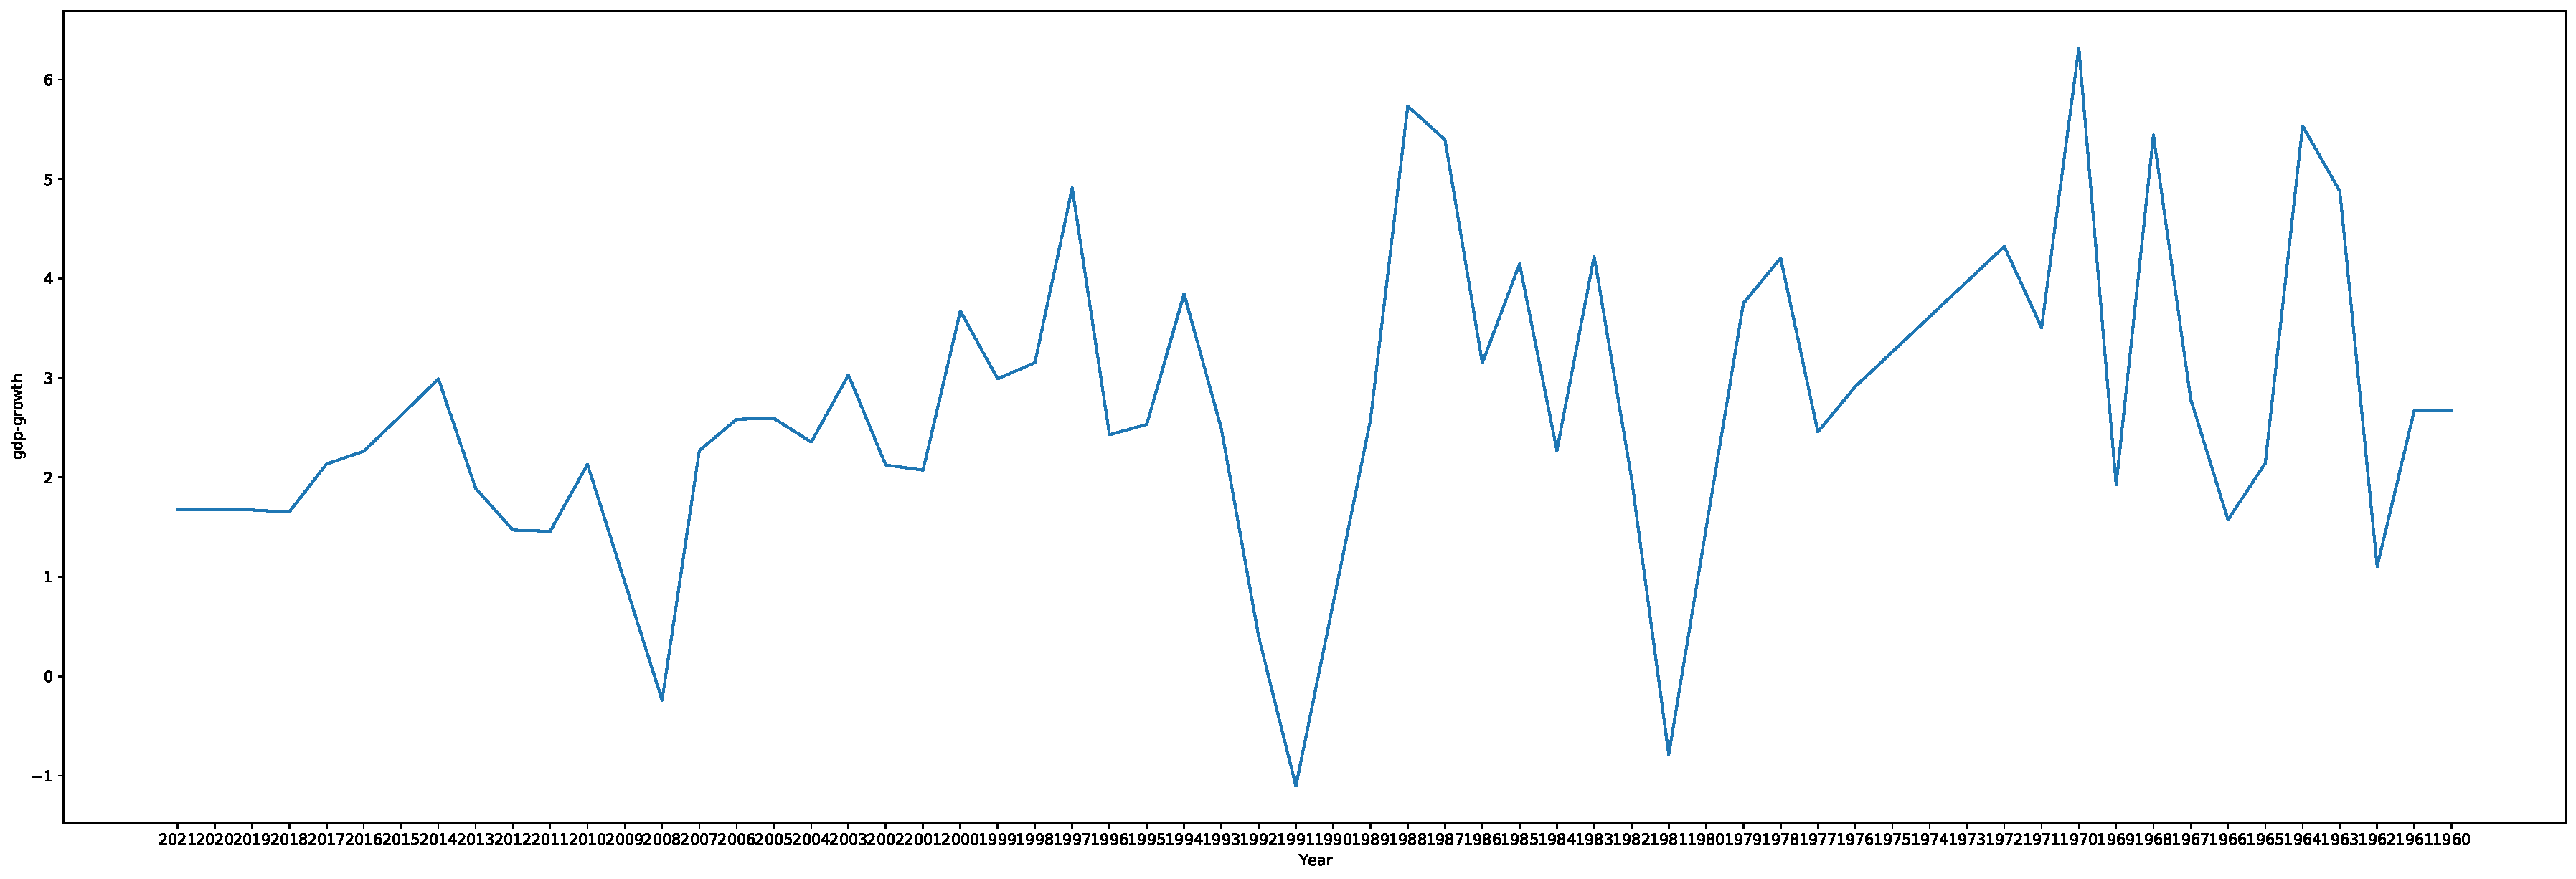
\includegraphics[width=0.7\textwidth]{Images/gdp-growth vs Year.pdf}
    \caption{GDP Growth}
    \label{fig1}
\end{figure}


\begin{figure}[H]
    \centering
    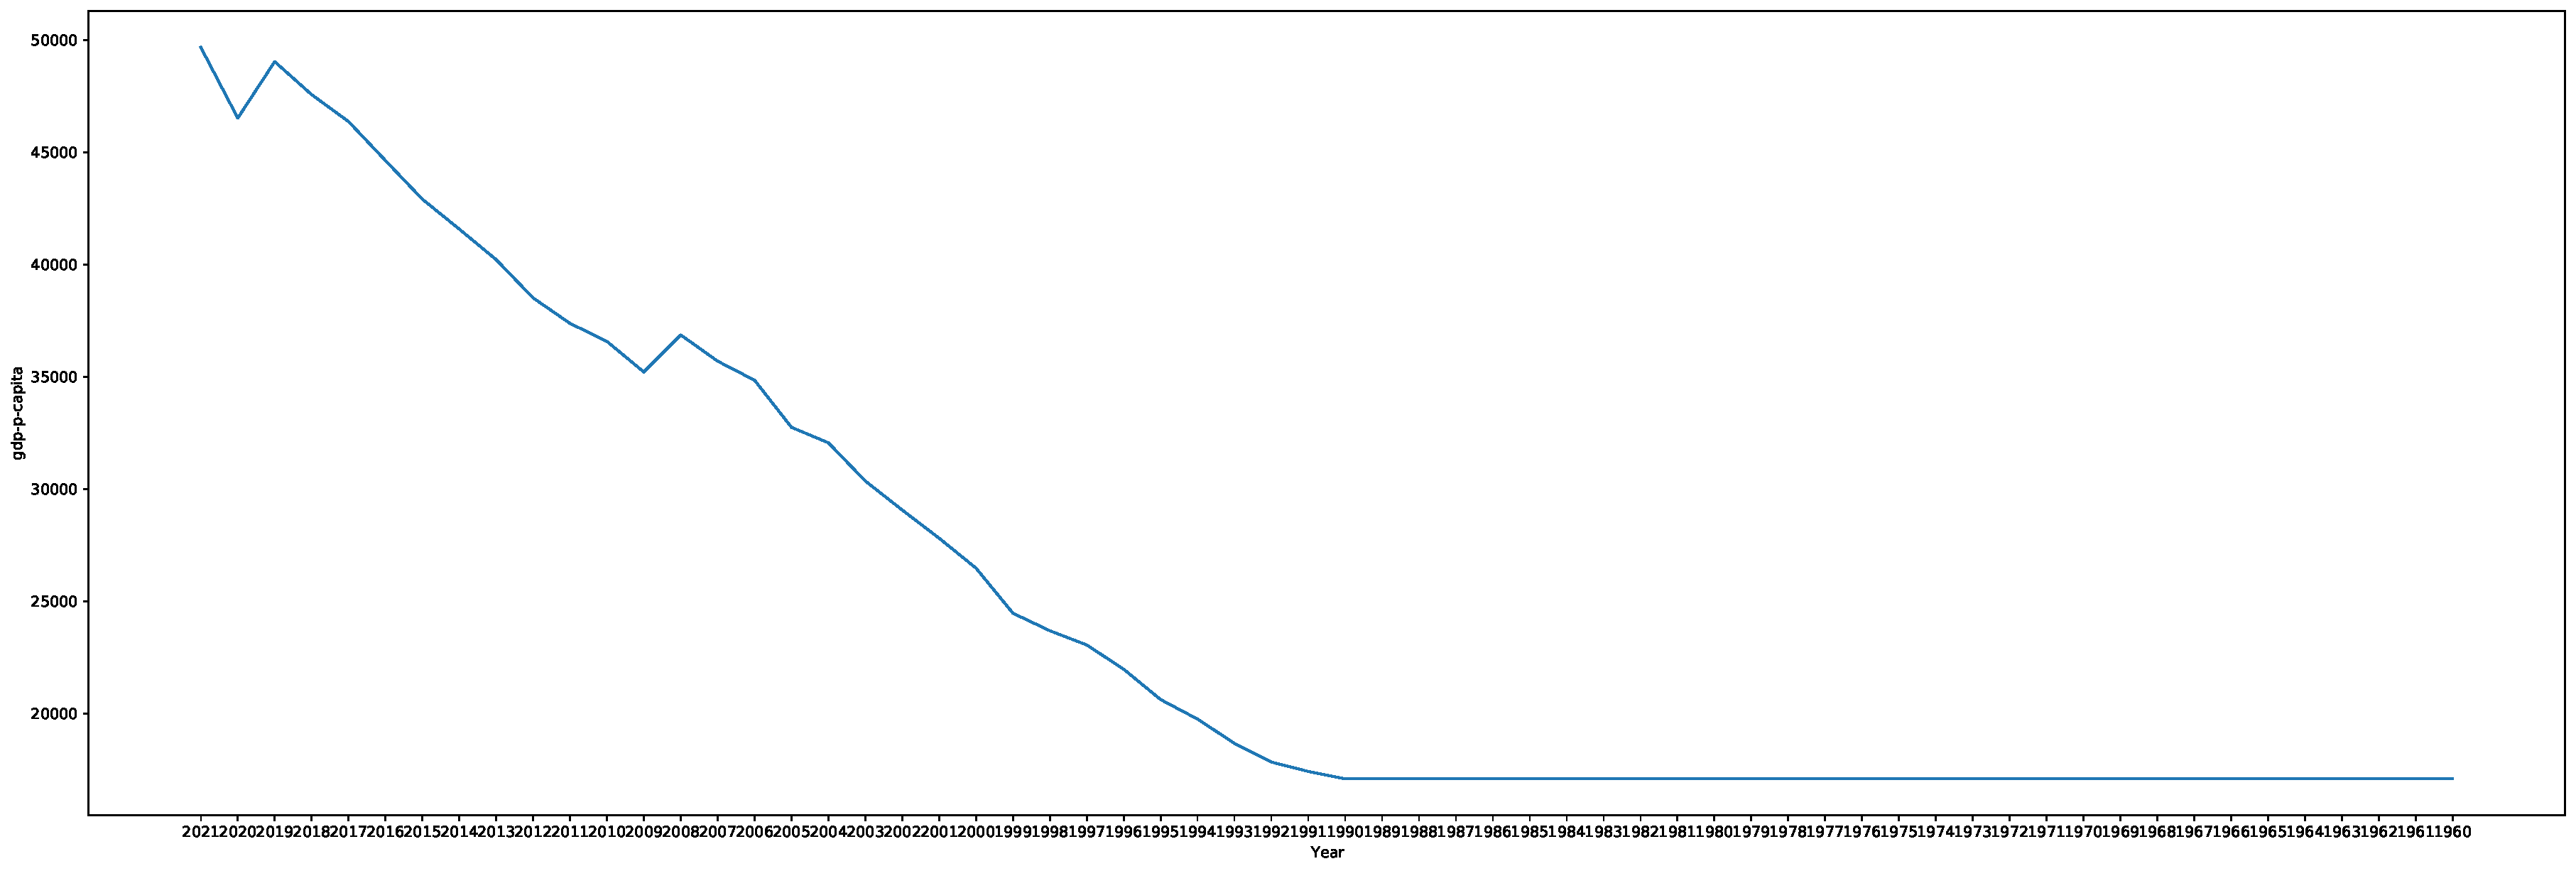
\includegraphics[width=0.7\textwidth]{Images/gdp-p-capita vs Year.pdf}
    \caption{GDP Person Capita}
    \label{fig1}
\end{figure}

\begin{figure}[H]
    \centering
    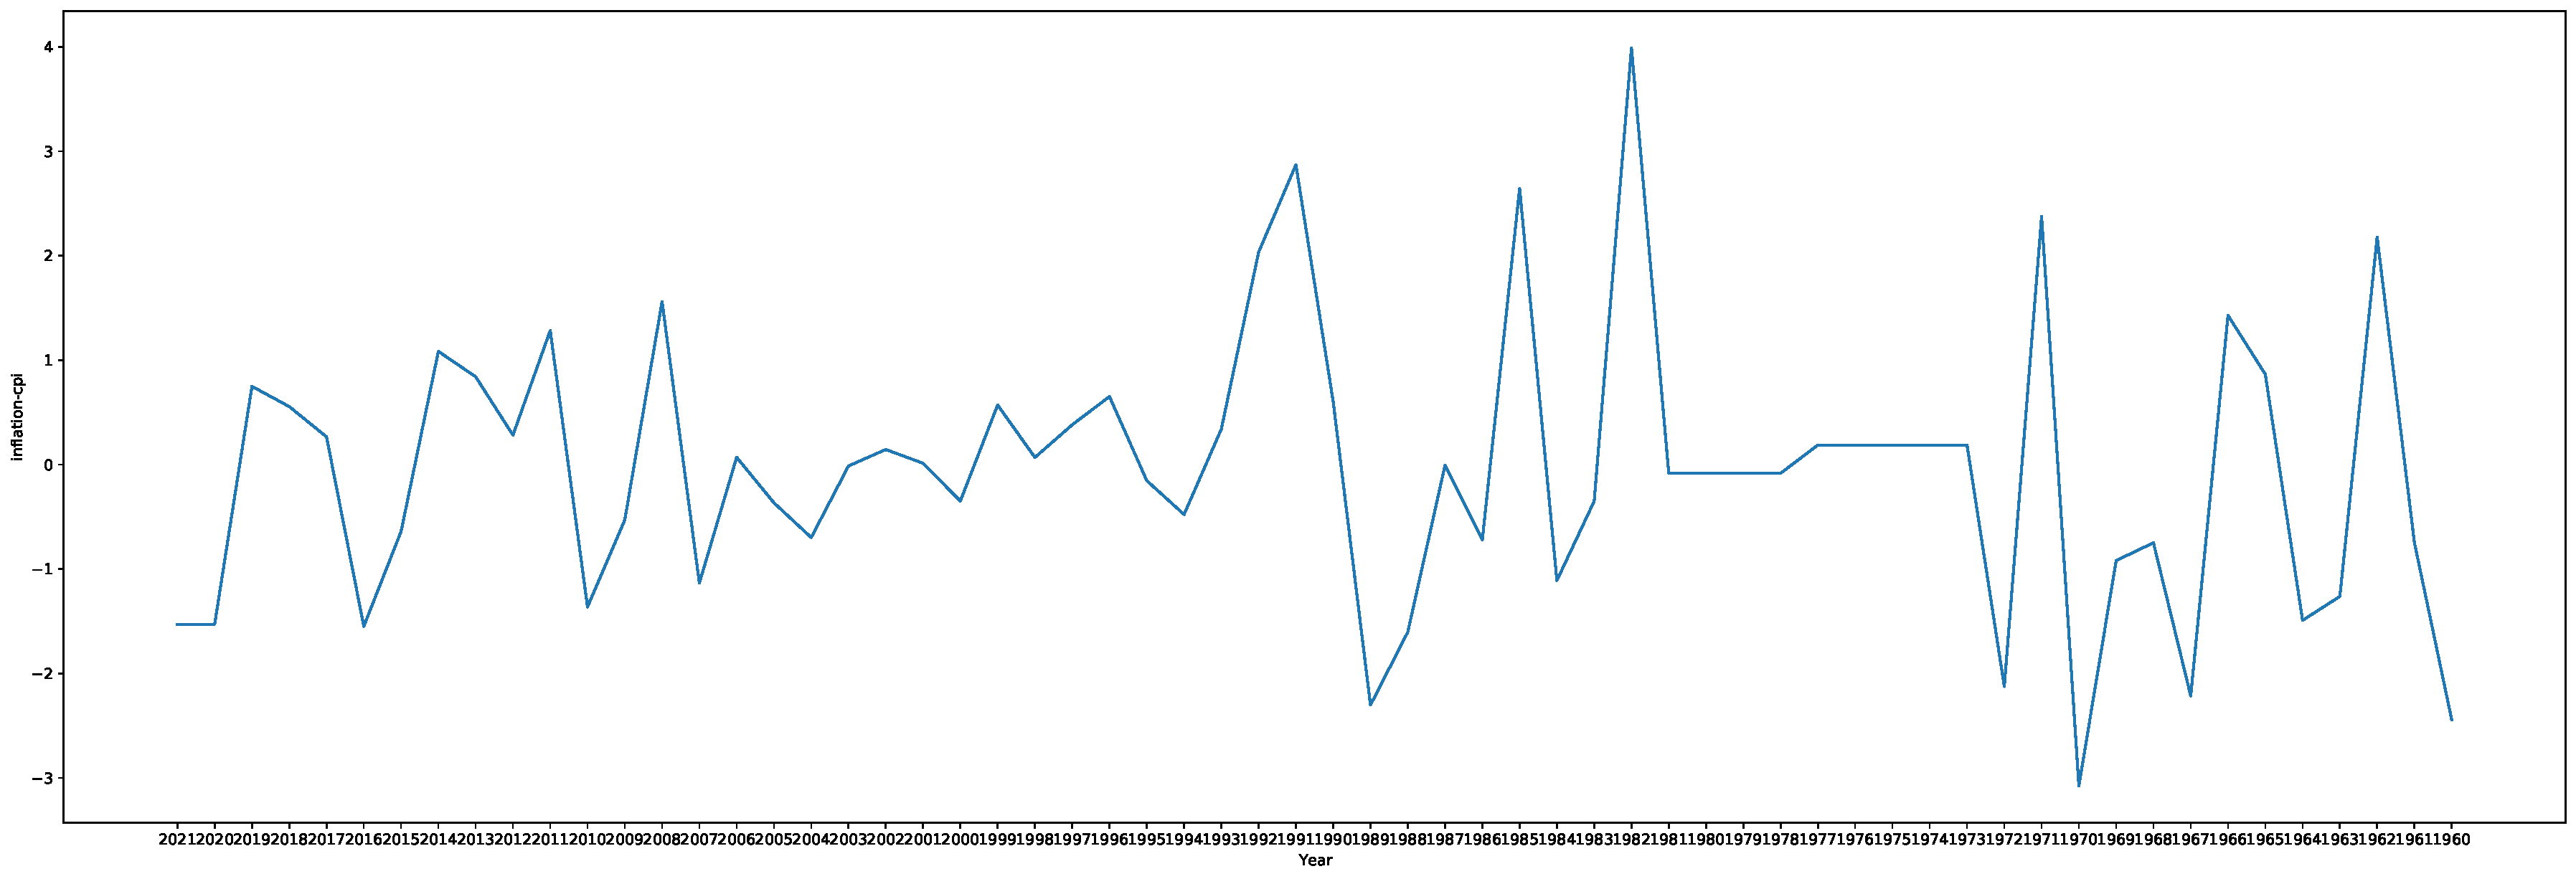
\includegraphics[width=0.7\textwidth]{Images/inflation-cpi vs Year.pdf}
    \caption{Inflation}
    \label{fig1}
\end{figure}

\begin{figure}[H]
    \centering
    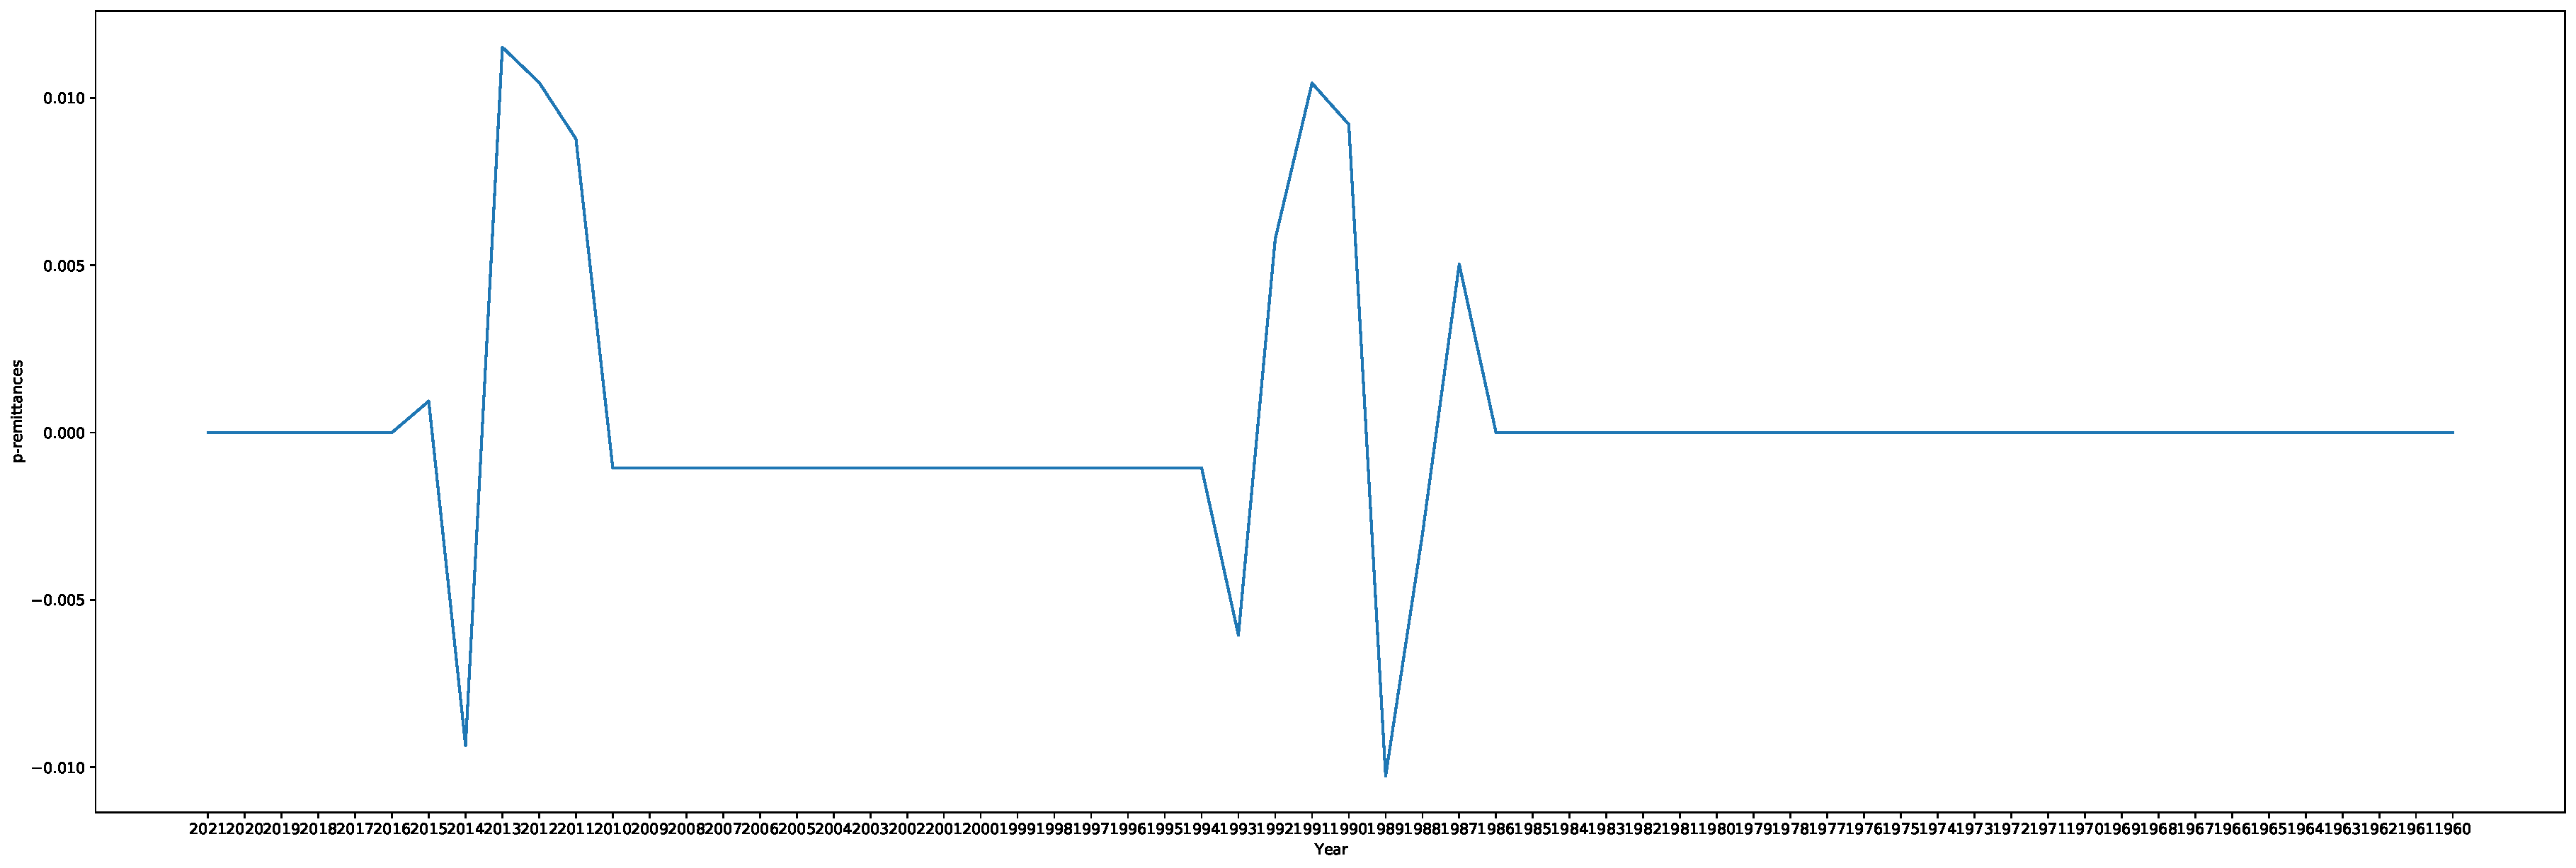
\includegraphics[width=0.7\textwidth]{Images/p-remittances vs Year.pdf}
    \caption{Personal remittances, received}
    \label{fig1}
\end{figure}

\begin{figure}[H]
    \centering
    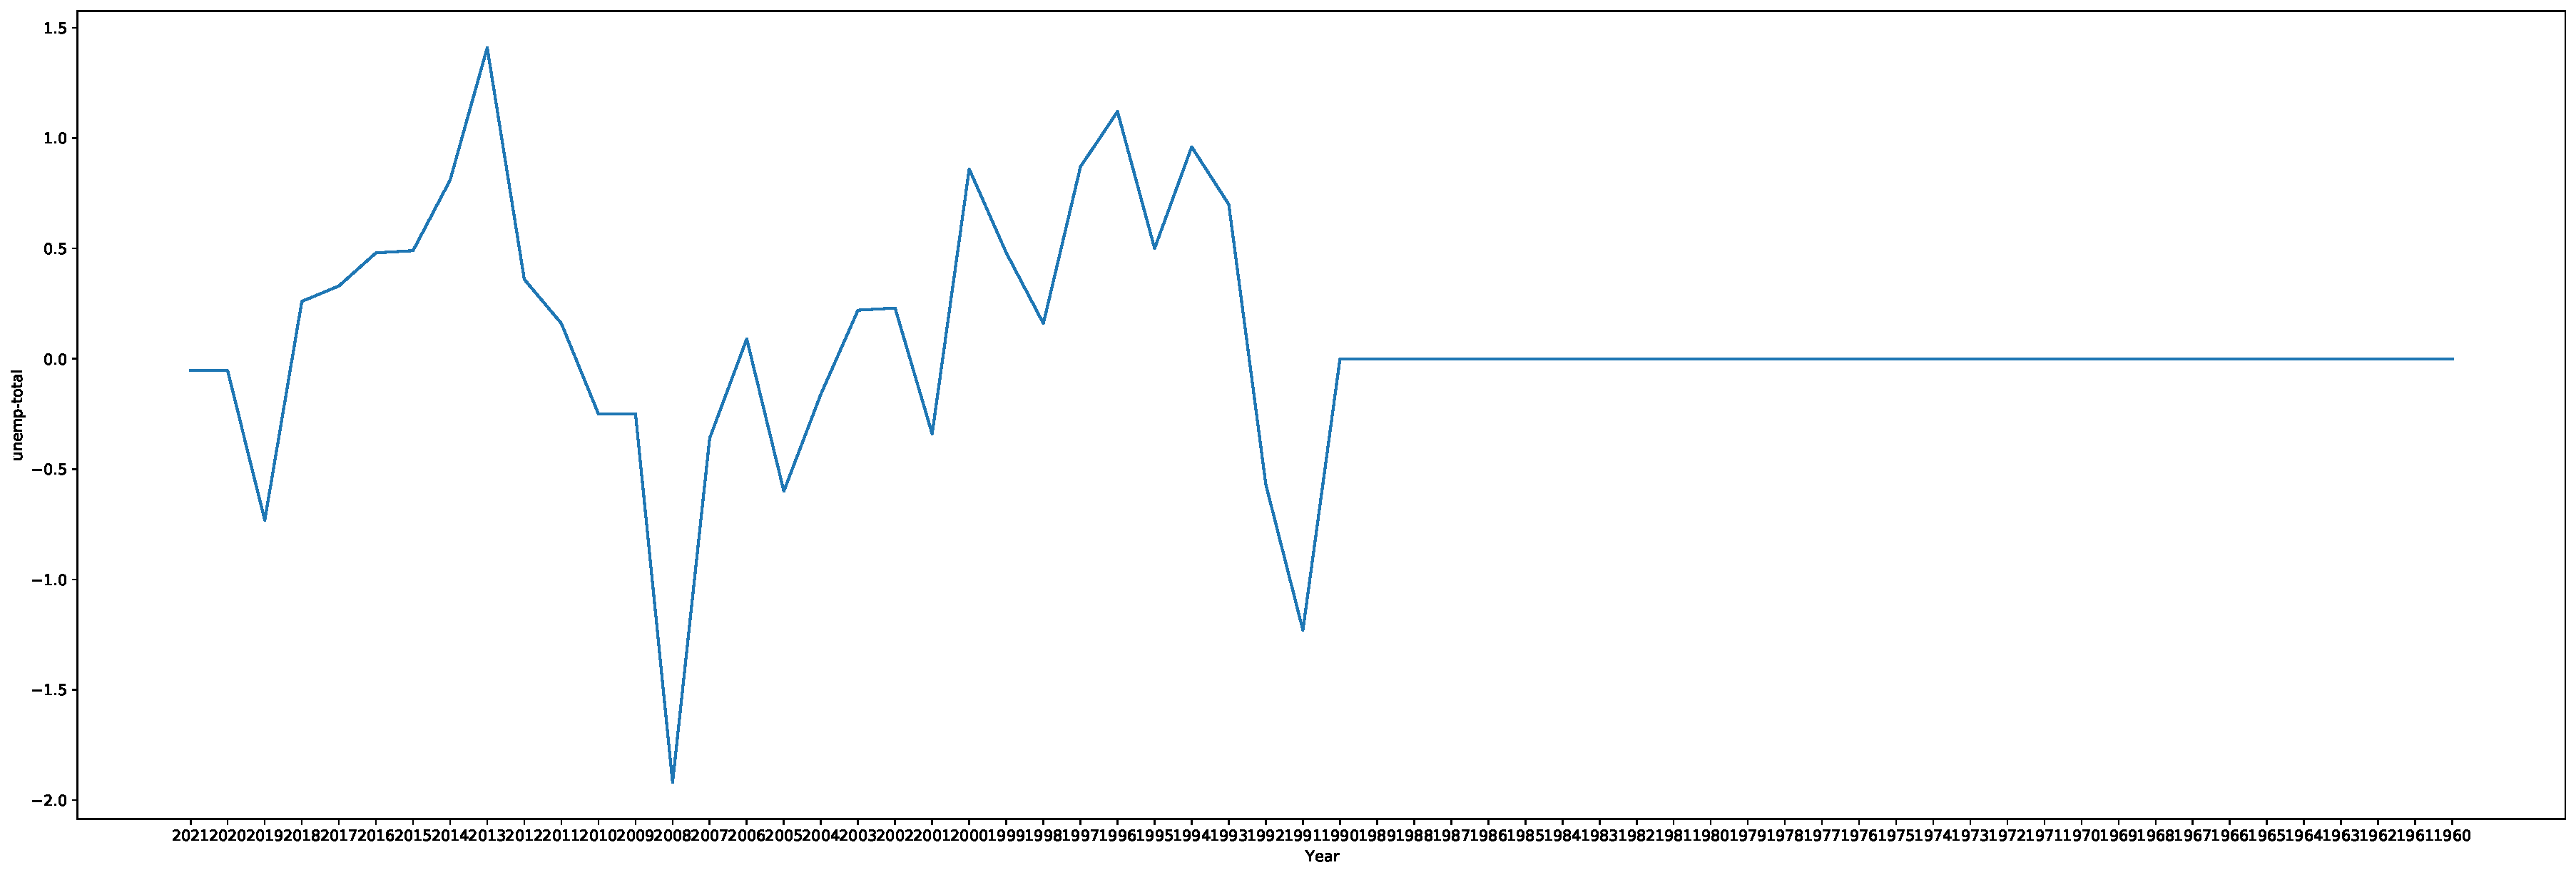
\includegraphics[width=0.7\textwidth]{Images/unemp-total vs Year.pdf}
    \caption{Unemployment}
    \label{fig1}
\end{figure}

Now we are done with pre-processing and data is ready for model training and testing.
